\documentclass[10pt]{article}
\usepackage[margin=1in]{geometry}
\usepackage[utf8]{inputenc}
\usepackage{multicol}
\setlength{\columnsep}{1mm}
\usepackage{amsfonts}
\usepackage{booktabs}
\usepackage{siunitx}
\usepackage[authoryear,round]{natbib}
\usepackage{float}
\usepackage[font={small}]{caption}
\usepackage[labelfont=bf]{caption}
\usepackage{lineno}
\usepackage{amsmath,amssymb,setspace,fancyhdr,geometry,url,color}
\usepackage{subfigure,graphicx,caption}
\usepackage{lscape,amsthm}
\usepackage{blindtext}
\usepackage{hhline}
\usepackage{arydshln}
\usepackage{verbatim}
\usepackage{dblfloatfix}
\usepackage{multirow}
\usepackage{graphicx}
\usepackage{xr}
\externaldocument{../PhaseIIPaper/main}
%\biboptions{authoryear, comma}
%%%%%%%%%%%%%%%%%%%%%%%%%%%%%%%%%%%%%%%%%%%%%%%%%%%%%%%%%%%%%%%%%%%%%%%%%
%%%%%%%%%%%%%%%%%%%%%%%%%%%%%%%%%%%%%%%%%%%%%%%%%%%%%%%%%%%%%%%%%%%%%%%%%%
\begin{document}
\centering{\bf {\large Supplemental Material} \\
{\Large The GGCMI Phase II experiment: simulating and emulating global crop yield responses to changes in carbon dioxide, temperature, water, and nitrogen levels}}\\

\vspace{3mm}

\centering{James Franke$^{1, 2}$, 
Joshua Elliott$^{2, 3}$, 
Christoph M\"{u}ller$^4$, 
Alexander Ruane$^5$, 
Abigail Snyder$^6$,\\ 
Jonas J\"{a}germeyr$^{3, 2, 4, 5}$, 
Juraj Balkovic$^{7, 8}$, 
Philippe Ciais$^{9, 10}$, 
Marie Dury$^{11}$, 
Pete Falloon$^{12}$,\\ 
Christian Folberth$^7$, 
Louis Fran{\c{c}}ois$^{11}$, 
Tobias Hank$^{13}$, 
Munir Hoffmann$^{14,23}$, 
Cesar Izaurralde$^{15, 16}$,\\ 
Ingrid Jacquemin$^11$, 
Curtis Jones$^{15}$, 
Nikolay Khabarov$^7$, 
Marian Koch$^{14}$, 
Michelle Li$^{2, 17}$, 
Wenfeng Liu$^{18, 9}$,\\ 
Stefan Olin$^{19}$, 
Meridel Phillips$^{5, 20}$, 
Thomas Pugh$^{21, 22}$, 
Ashwan Reddy$^{15}$, 
Xuhui Wang$^{9, 10}$,\\ 
Karina Williams$^{12}$, 
Florian Zabel$^{13}$, 
and Elisabeth Moyer$^{1, 2}$\\
~\\}

\centering{
{\small 1.  Department of the Geophysical Sciences, University of Chicago, Chicago, IL, USA}\\
{\small 2.  Center for Robust Decision-making on Climate and Energy Policy, University of Chicago, Chicago, IL, USA}\\
{\small 3.  Department of Computer Science, University of Chicago, Chicago, IL, USA}\\
{\small 4.  Potsdam Institute for Climate Impact Research, Leibniz Association (Member), Potsdam, Germany}\\
{\small 5.  NASA Goddard Institute for Space Studies, New York, NY, United States}\\
{\small 6.  Joint Global Change Research Institute, Pacific Northwest National Laboratory, College Park, MD, USA}\\
{\small 7.  Ecosystem Services and Mgm. Prg., International Institute for Applied Systems Analysis, Laxenburg, Austria}\\
{\small 8.  Department of Soil Science, Comenius University in Bratislava, Bratislava, Slovak Republic}\\
{\small 9.  Laboratoire des Sciences du Climat et de l'Environnement,CEA-CNRS-UVSQ, 91191 Gif-sur-Yvette, France}\\
{\small 10. Sino-French Institute of Earth System Sciences, Peking University, Beijing, China}\\
{\small 11. Unit{\'{e}} de Mod{\'{e}}lisation du Climat et des Cycles Biog\'eochimiques, University of Li\`ege, Belgium}\\
{\small 12. Met Office Hadley Centre, Exeter, United Kingdom}\\
{\small 13. Department of Geography, Ludwig-Maximilians-Universit\"{a}t, Munich, Germany}\\
{\small 14. Georg-August-University G\"{o}ttingen, Tropical Plant Production and Ag. Sys. Modelling, G\"{o}ttingen, Germany}\\
{\small 15. Department of Geographical Sciences, University of Maryland, College Park, MD, USA}\\
{\small 16. Texas Agrilife Research and Extension, Texas A\&M University, Temple, TX, USA}\\
{\small 17. Department of Statistics, University of Chicago, Chicago, IL, USA}\\
{\small 18. EAWAG, Swiss Federal Institute of Aquatic Science and Technology, D\"{u}bendorf, Switzerland}\\
{\small 19. Department of Physical Geography and Ecosystem Science, Lund University, Lund, Sweden}\\
{\small 20. Earth Institute Center for Climate Systems Research, Columbia University, New York, NY, USA}\\
{\small 21. Karlsruhe Institute of Technology, IMK-IFU, 82467 Garmisch-Partenkirchen, Germany}\\
{\small 22. School of Geography, Earth and Environmental Science, University of Birmingham, Birmingham, UK}\\
{\small 23. Leibniz Centre for Agricultural Landscape Research (ZALF), D-15374 Müncheberg, Germany}
}

\tableofcontents

%%%%%%%%%%%%%%%%%%%%%%%%%%%%%%%%%%%
\clearpage
\modulolinenumbers[2]
\linenumbers
%%%%%%%%%%%%%%%%%%%%%%%%%%%%%%%%%%%

\renewcommand{\thefigure}{S\arabic{figure}}

\section{Methods}
Additional example figures for reference in the methods section as noted in the manuscript. Some manuscript figure also repeated for ease of comparison.

\begin{figure}[h!]
\centering
\begin{minipage}{.45\textwidth}
    \centering
    \vspace{0pt}
    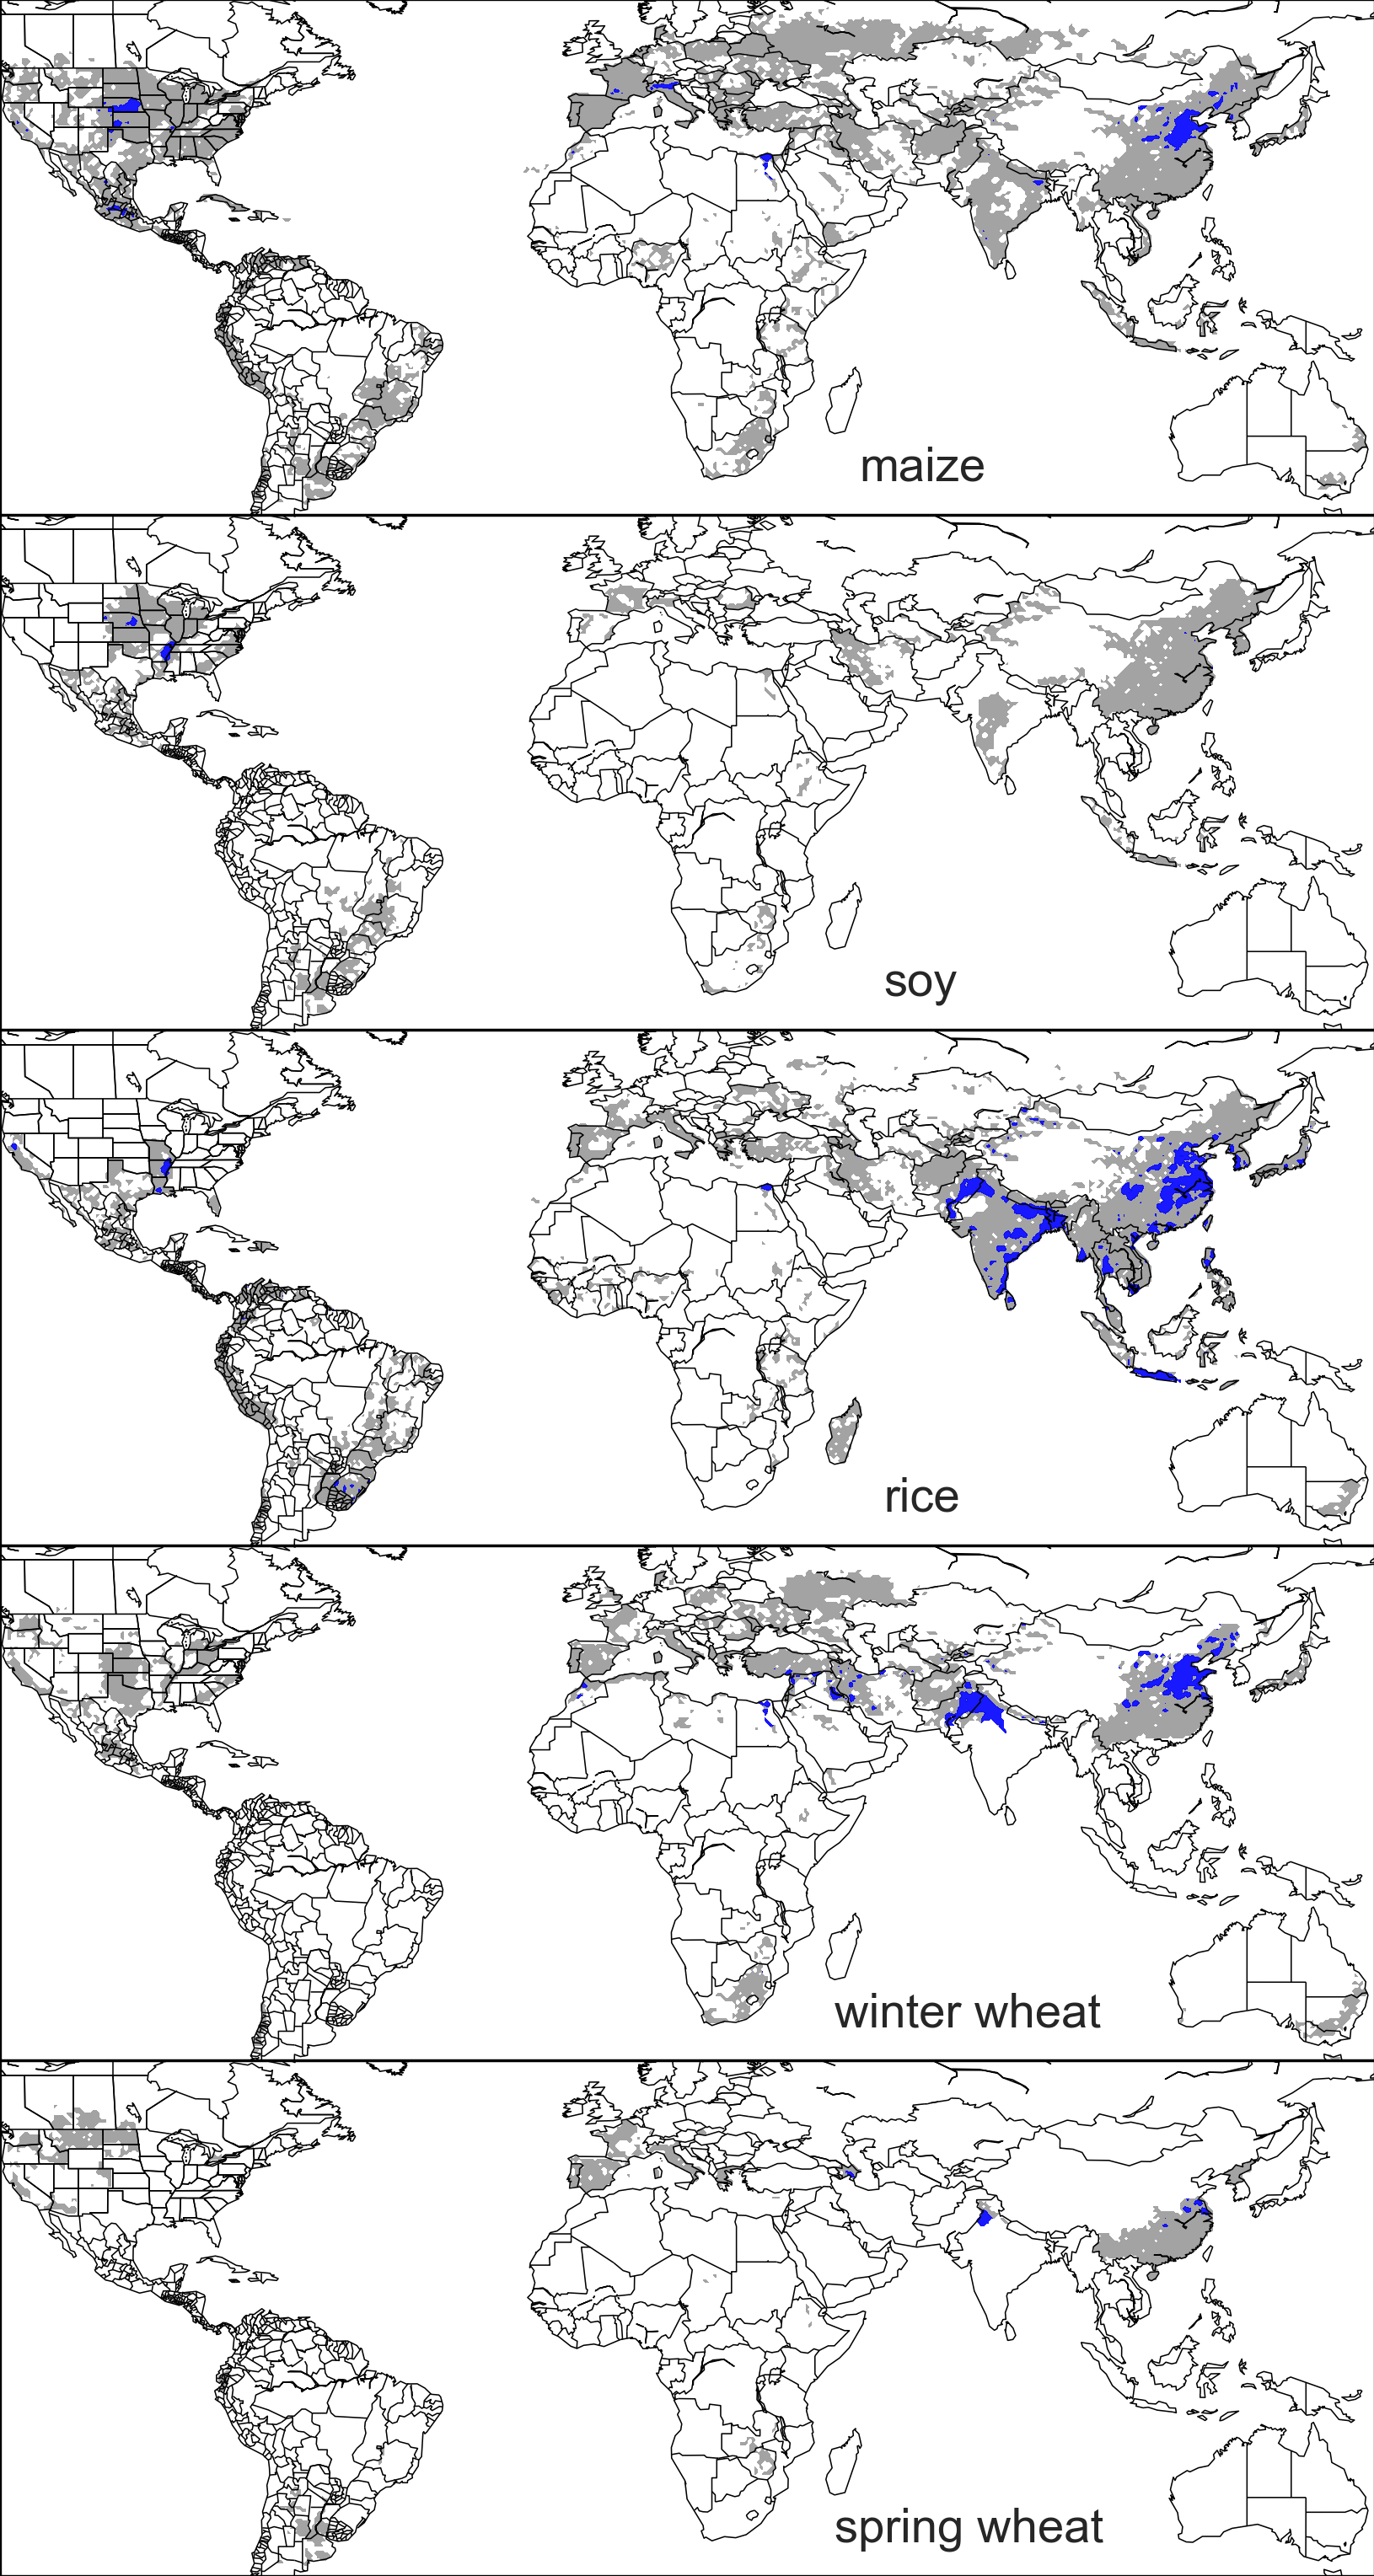
\includegraphics[width=\textwidth]{s_croparea_irr.png}\\
    \caption{Presently cultivated area for irrigated crops in the real world. The blue contour area indicates grid-cells with more that 20,00 hectares of crop cultivated. The gray contour shows area with more that 10 hectares cultivated. Data from the MIRCA2000 data set for maize, rice, and soy. Winter and spring wheat areas are adapted from MIRCA2000 data and sorted by growing season.}
    \label{fig:irrarea}
\end{minipage}
\hspace{.05\linewidth}
\begin{minipage}{.45\textwidth}
    \centering
    \vspace{-19mm}
    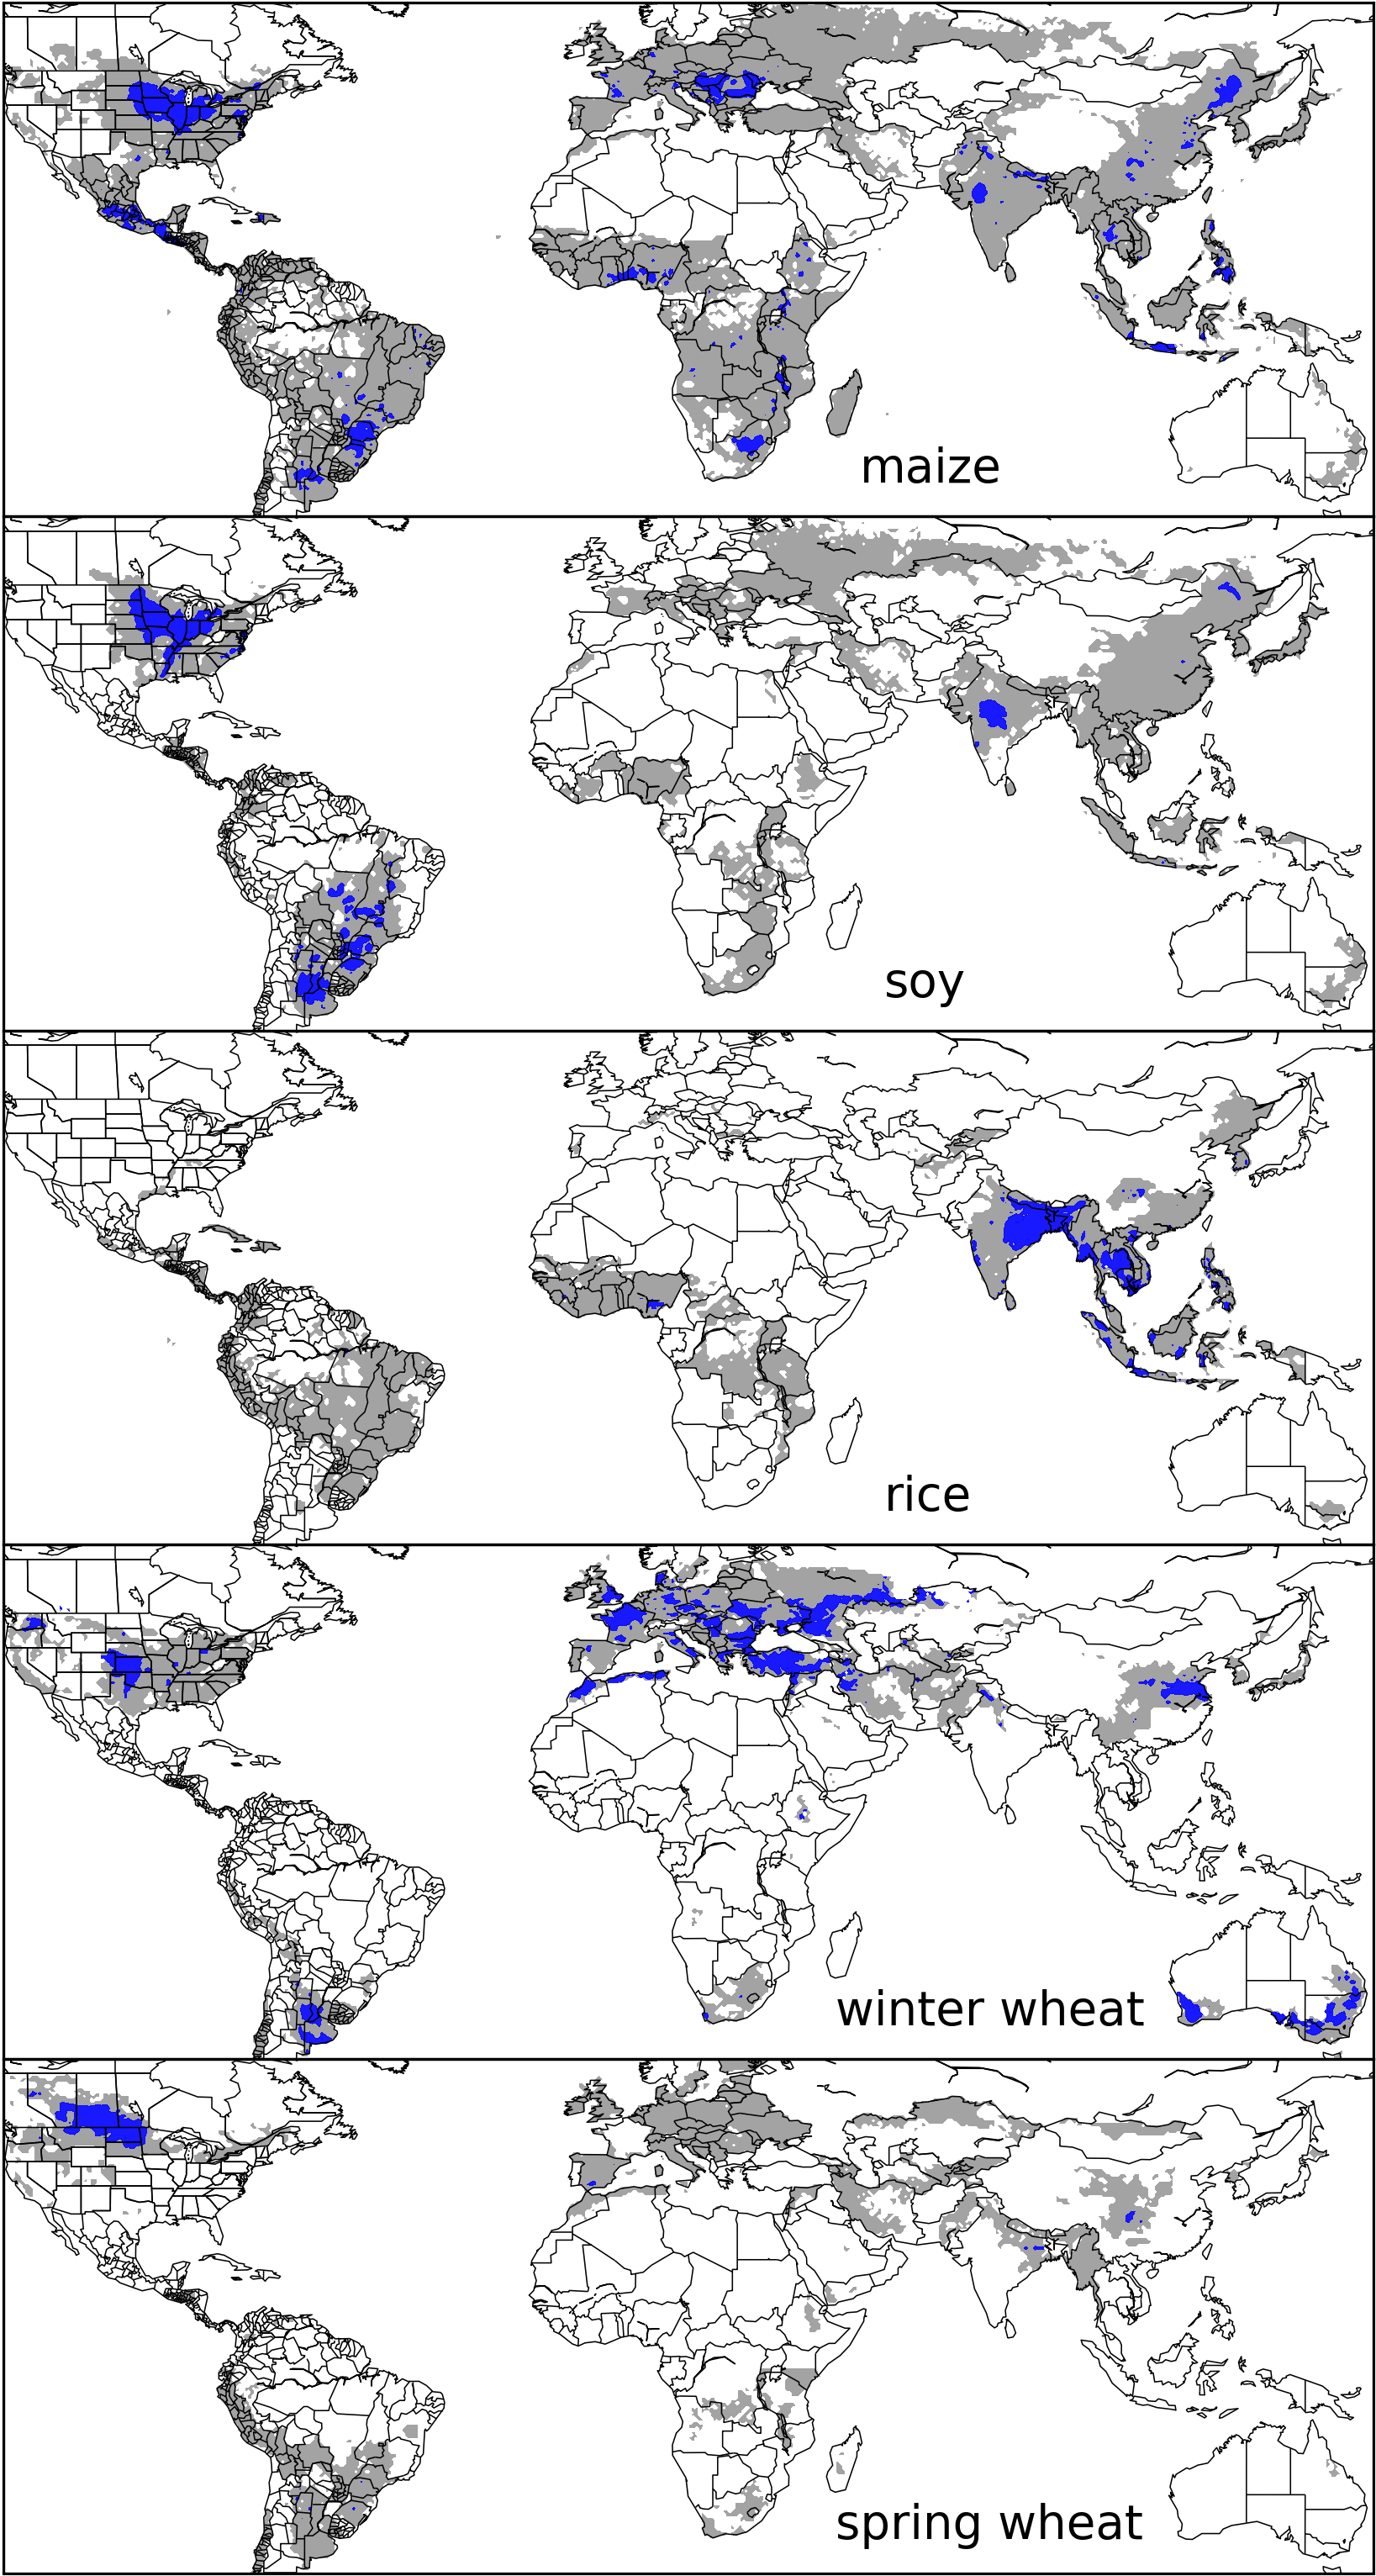
\includegraphics[width=\textwidth]{s_croparea.png}\\
    \caption{Presently cultivated area for rain fed crops in the real world. Conventions as in Figure S1. This figure repeats manuscript Figure 1.}
    \label{fig:rainfed}
\end{minipage}
\end{figure}

\begin{figure}[h!]
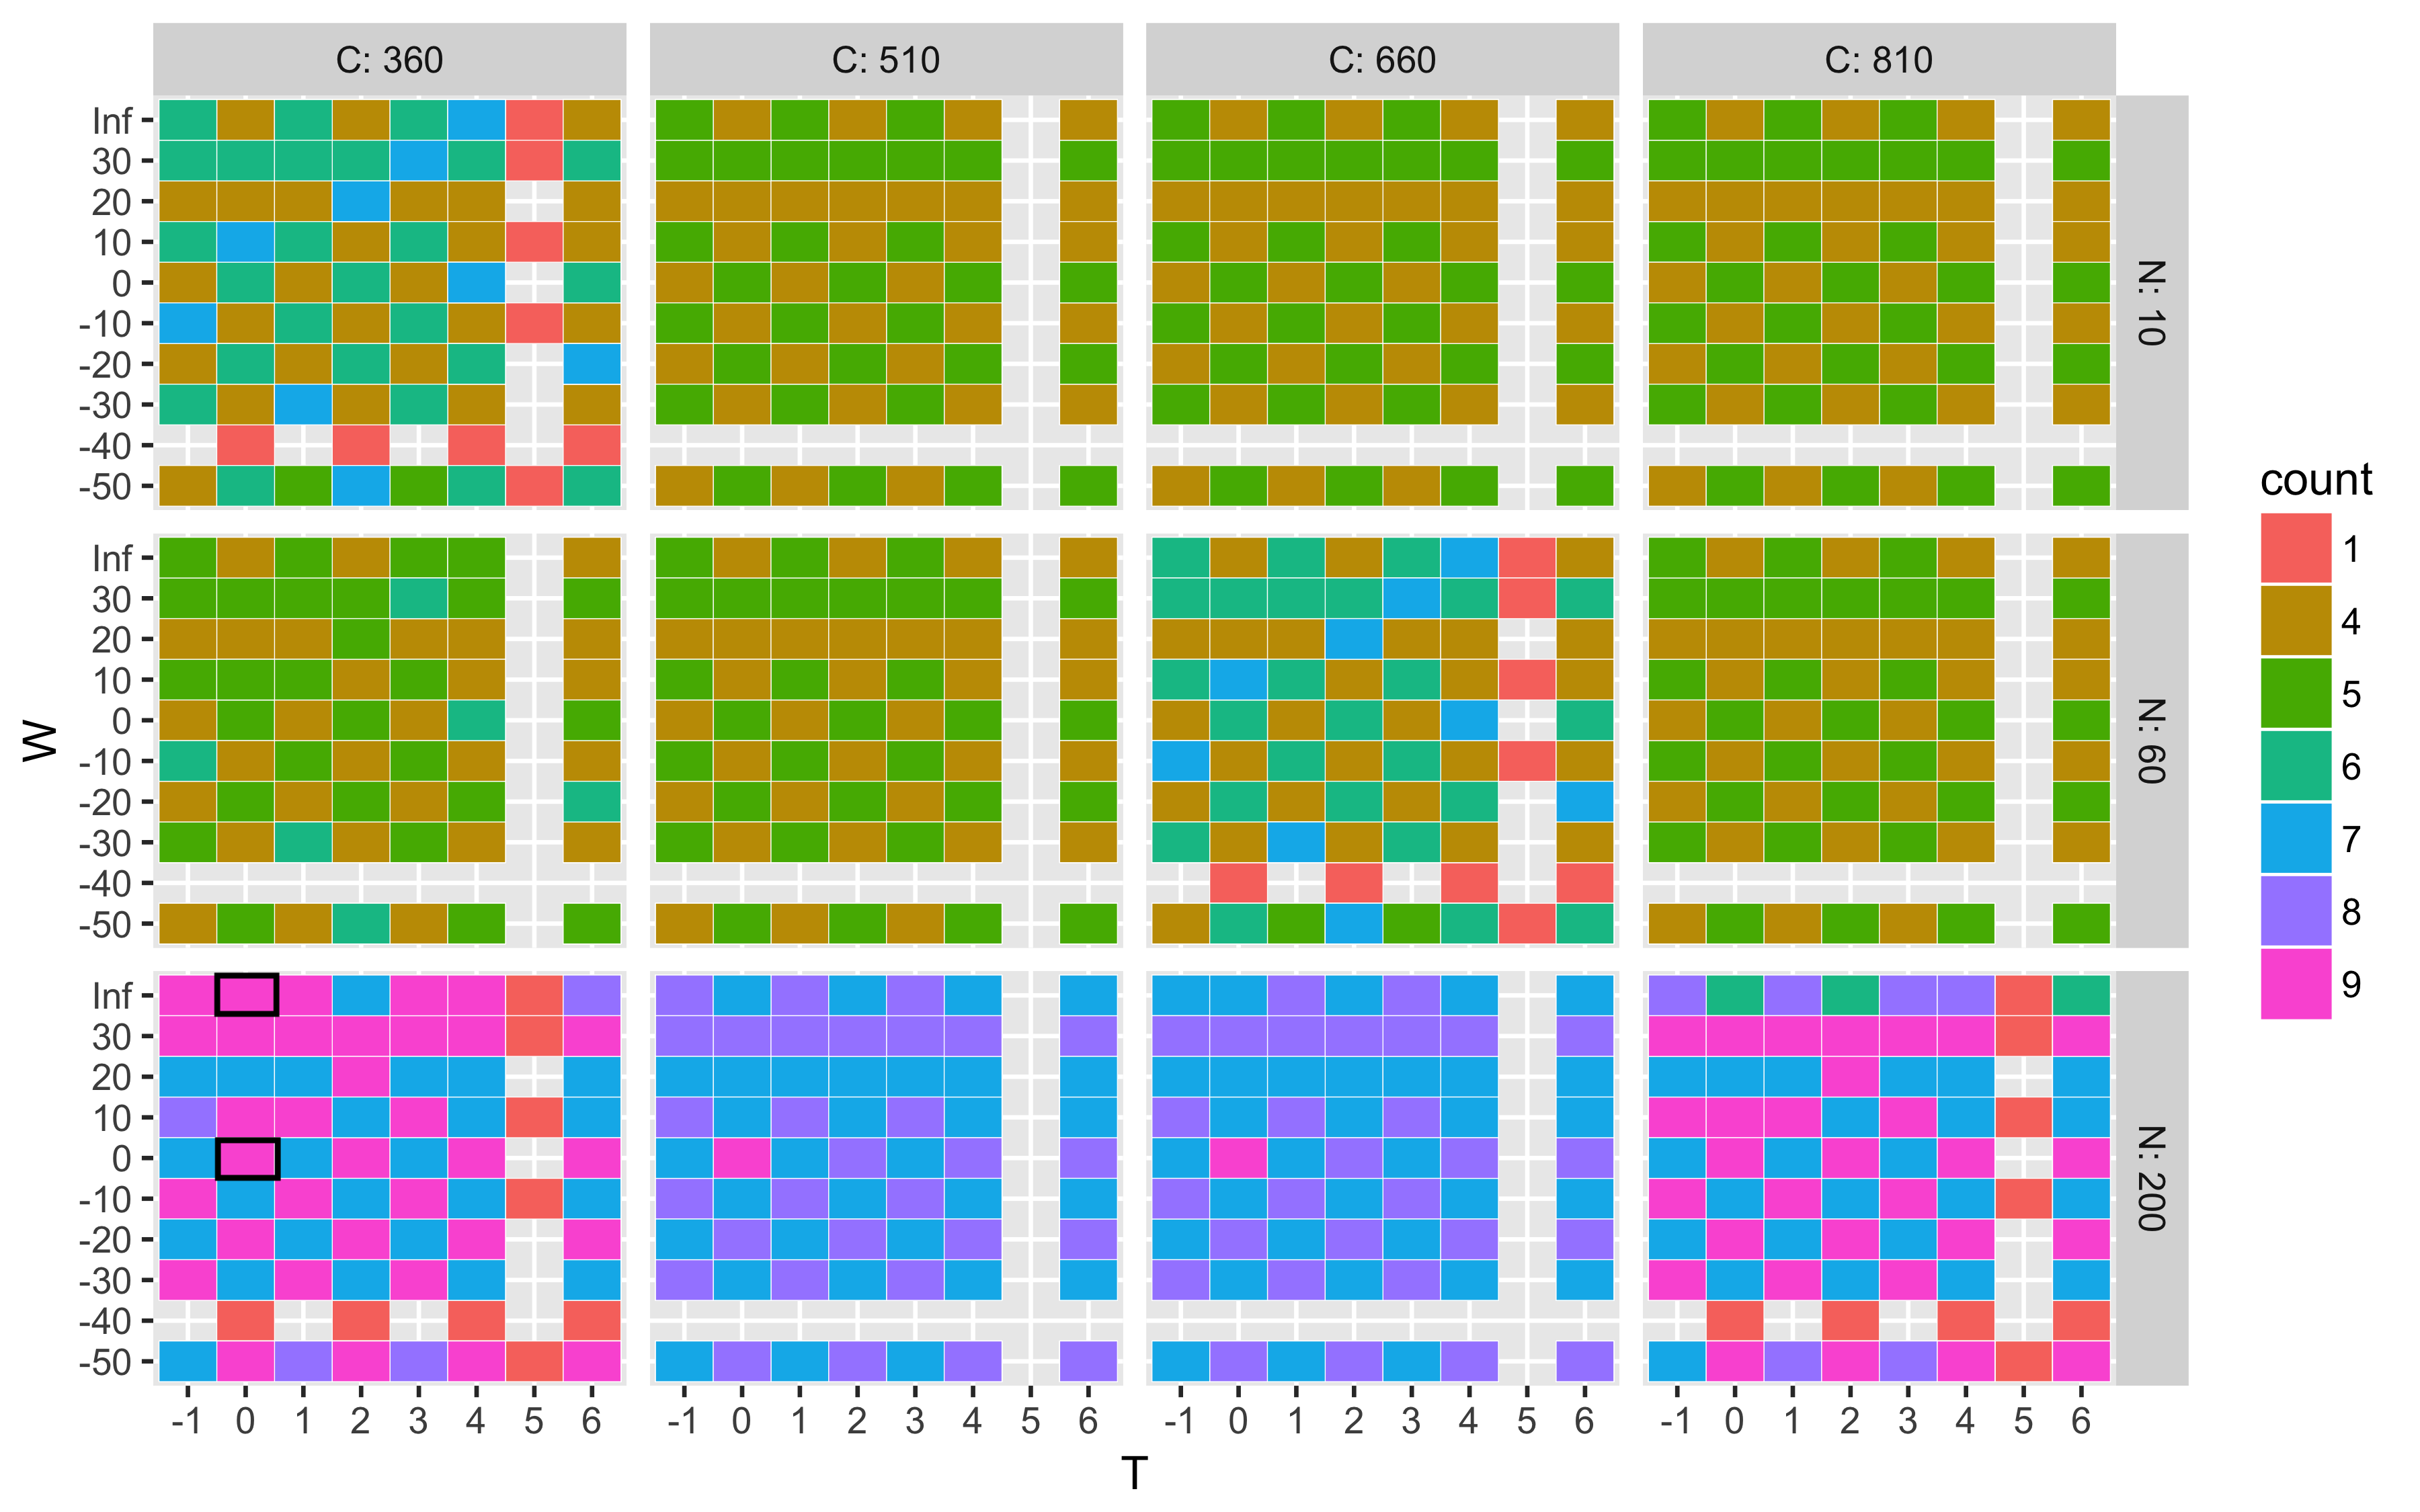
\includegraphics[width=\textwidth]{s_how_many_simulations.png}\\
\caption{Tile heatmap illustrates number of model simulations provided for each of the scenarios in the variable space. The max number is 9, the number of models included in the emulator analysis. Error calculations are run over scenarios where all models provided a simulation. Three models were excluded from the emulator analysis due to low sampling. Error calculations are run over scenarios with max number of models (See Figures \ref{fig:error360total}, \ref{fig:error810}.}
\label{fig:numbersims}
\end{figure}

\begin{figure}[h!]
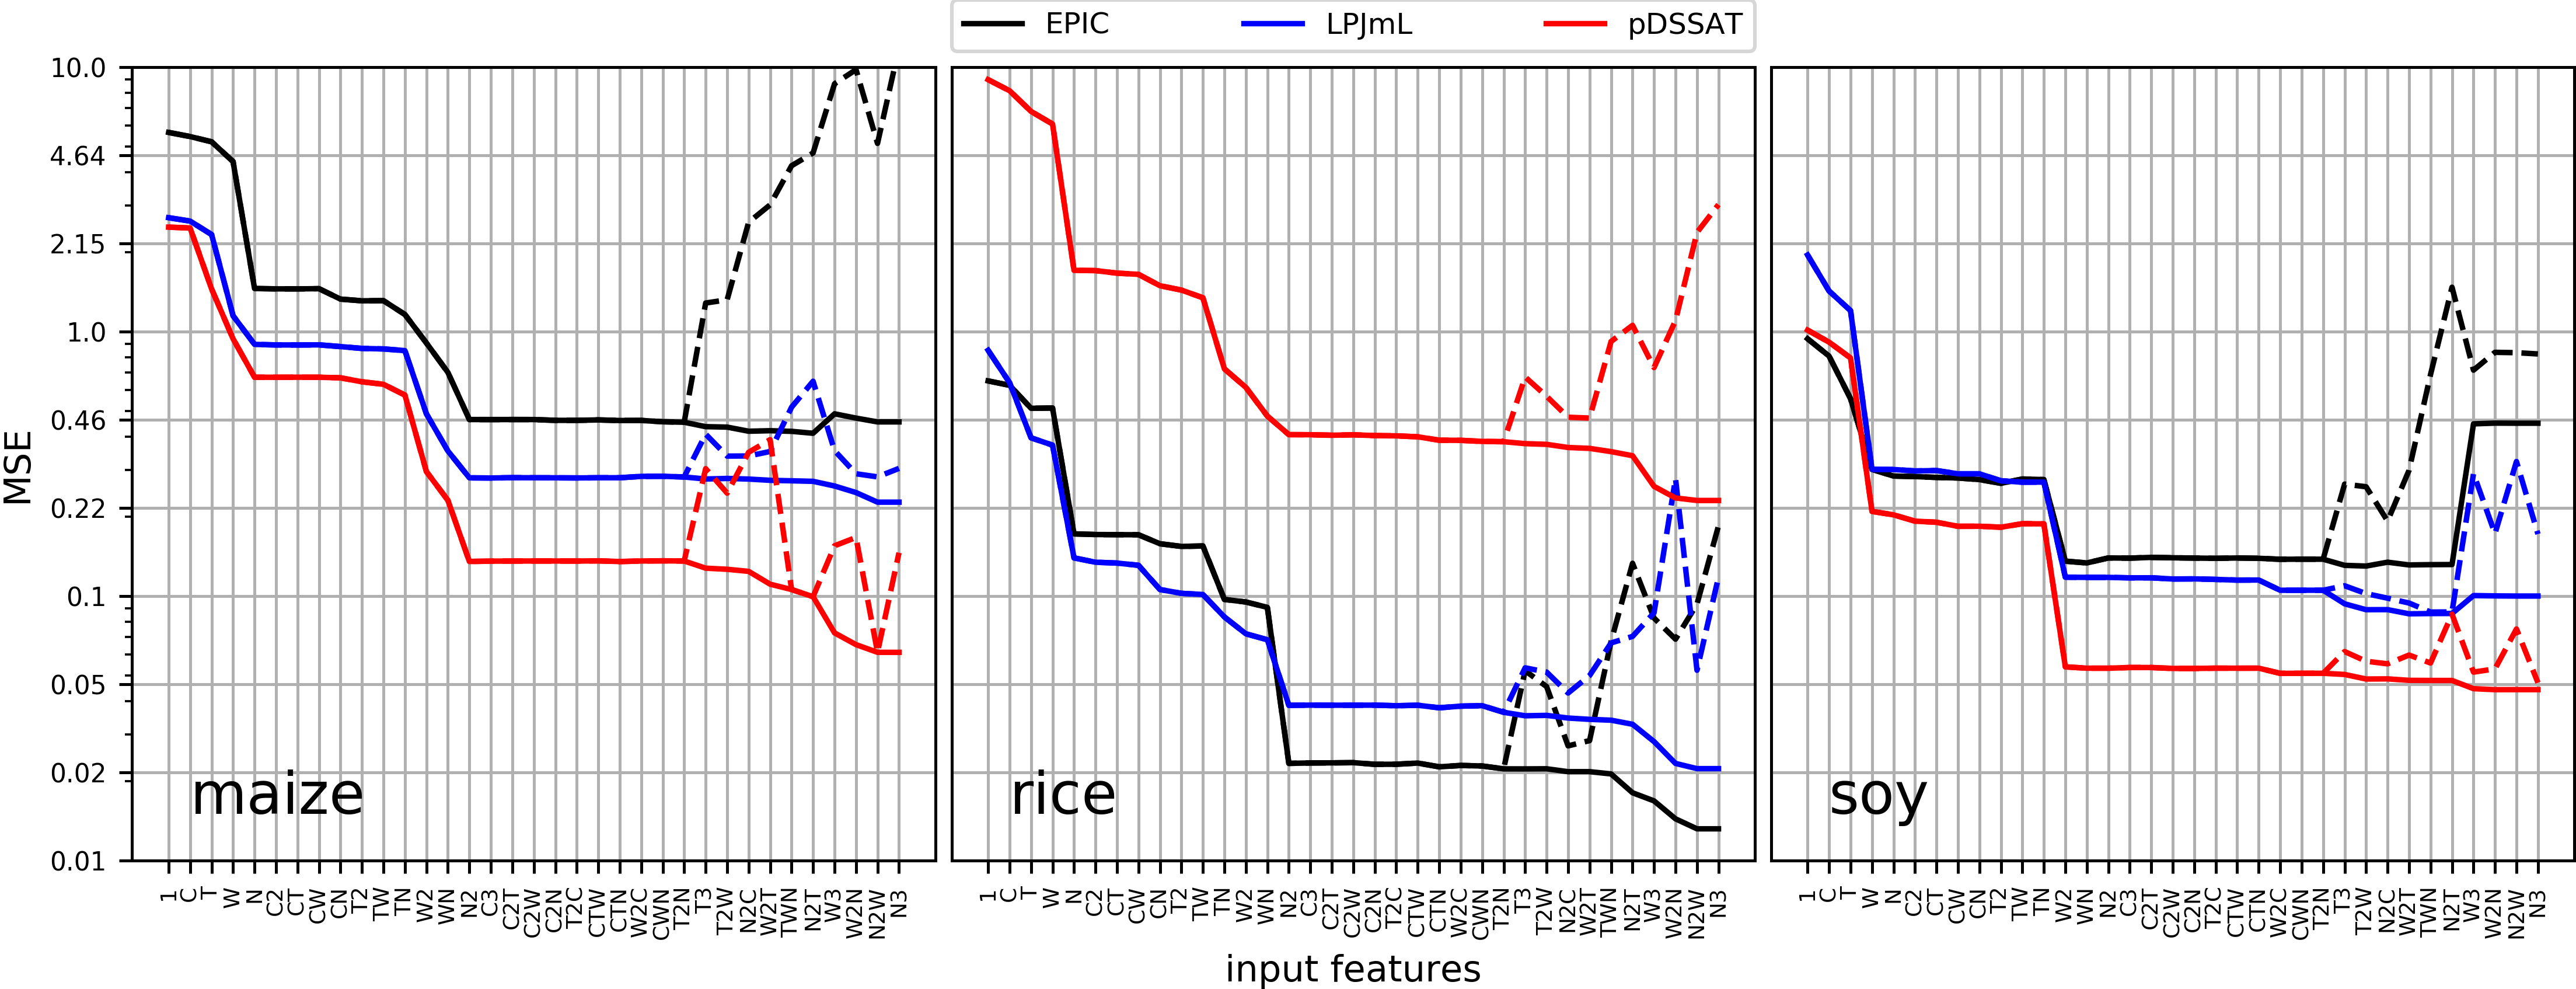
\includegraphics[width=\textwidth]{s_feature_selection.png}\\
\caption{Mean Squared Error (MSE) from the cross-validation process. The emulate yield for maize rice and soy are compared to the simulated values for the same model in all grid cells where crops are actually cultivated, weighted by area in each grid cell. X- axis indicates terms included in the model at each step progressively where T = temperature and T2 = temperature$^{2}$ and so on. Terms that did not reduce the aggregate error are not included in the final model. Some terms that did not reduce the aggregate error are included if a higher order version of that term provided a decrease in mean squared error (i.e. temperature cubed cannot be included without the temperature squared term, and the linear temperature term). Even though the models exhibit different absolute levels of error, all three models agree remarkably well on feature importance. Solid lines indicate L1 normalization and dashed lines indicate L2 normalization of yield outputs. Colors indicated different models (three fully-sampled simulation sets.)}
\label{fig:featureselection}
\end{figure}

\clearpage
\section{Simulation results}
We present additional simulation results for illustration as noted in the manuscript. 
%Most crops exhibit a somewhat uniform response to temperature increase across different K\"{o}ppen-Geiger when analyzed over currently cultivated area (see Figure \ref{fig:temperature}: i.e. equatorial maize and `snow' maize show similar response to a temperature increase). 
%This counterintuitive result agrees with existing literature including \citet{Rosenzweig2014} which shows increases in yields mainly in regions where crops are not currently grown and in \citet{Bassu2014}. A primary cause of this effect is less difference in growing season temperature across K\"{o}ppen-Geiger regions when they are weighted by current cultivation area than might be expected. Additionally, it has been proposed that the growing season is shortened under warmer temperatures in a way that is independent of baseline growing season temperature \citep[e.g.][]{Wang2017, Rezaei2018}. Currently most models in GGCMI include a direct linear shortening of the growing season with warming, but uncertainty about the exact nature of this response remains and it is an active area of research.

%The CO$_2$ response is generally subject to large uncertainties (not evident in Figures \ref{fig:regression} -- \ref{fig:regression_iowa} for maize as it is a C4 crop). All relevant CO$_2$ processes have not been studied in sufficient detail or have not been implemented in models sufficiently \citep[e.g.][]{Boote13} and a broader experimental basis for model parameterization is needed \citep{leaky09}

\begin{figure}[h!]
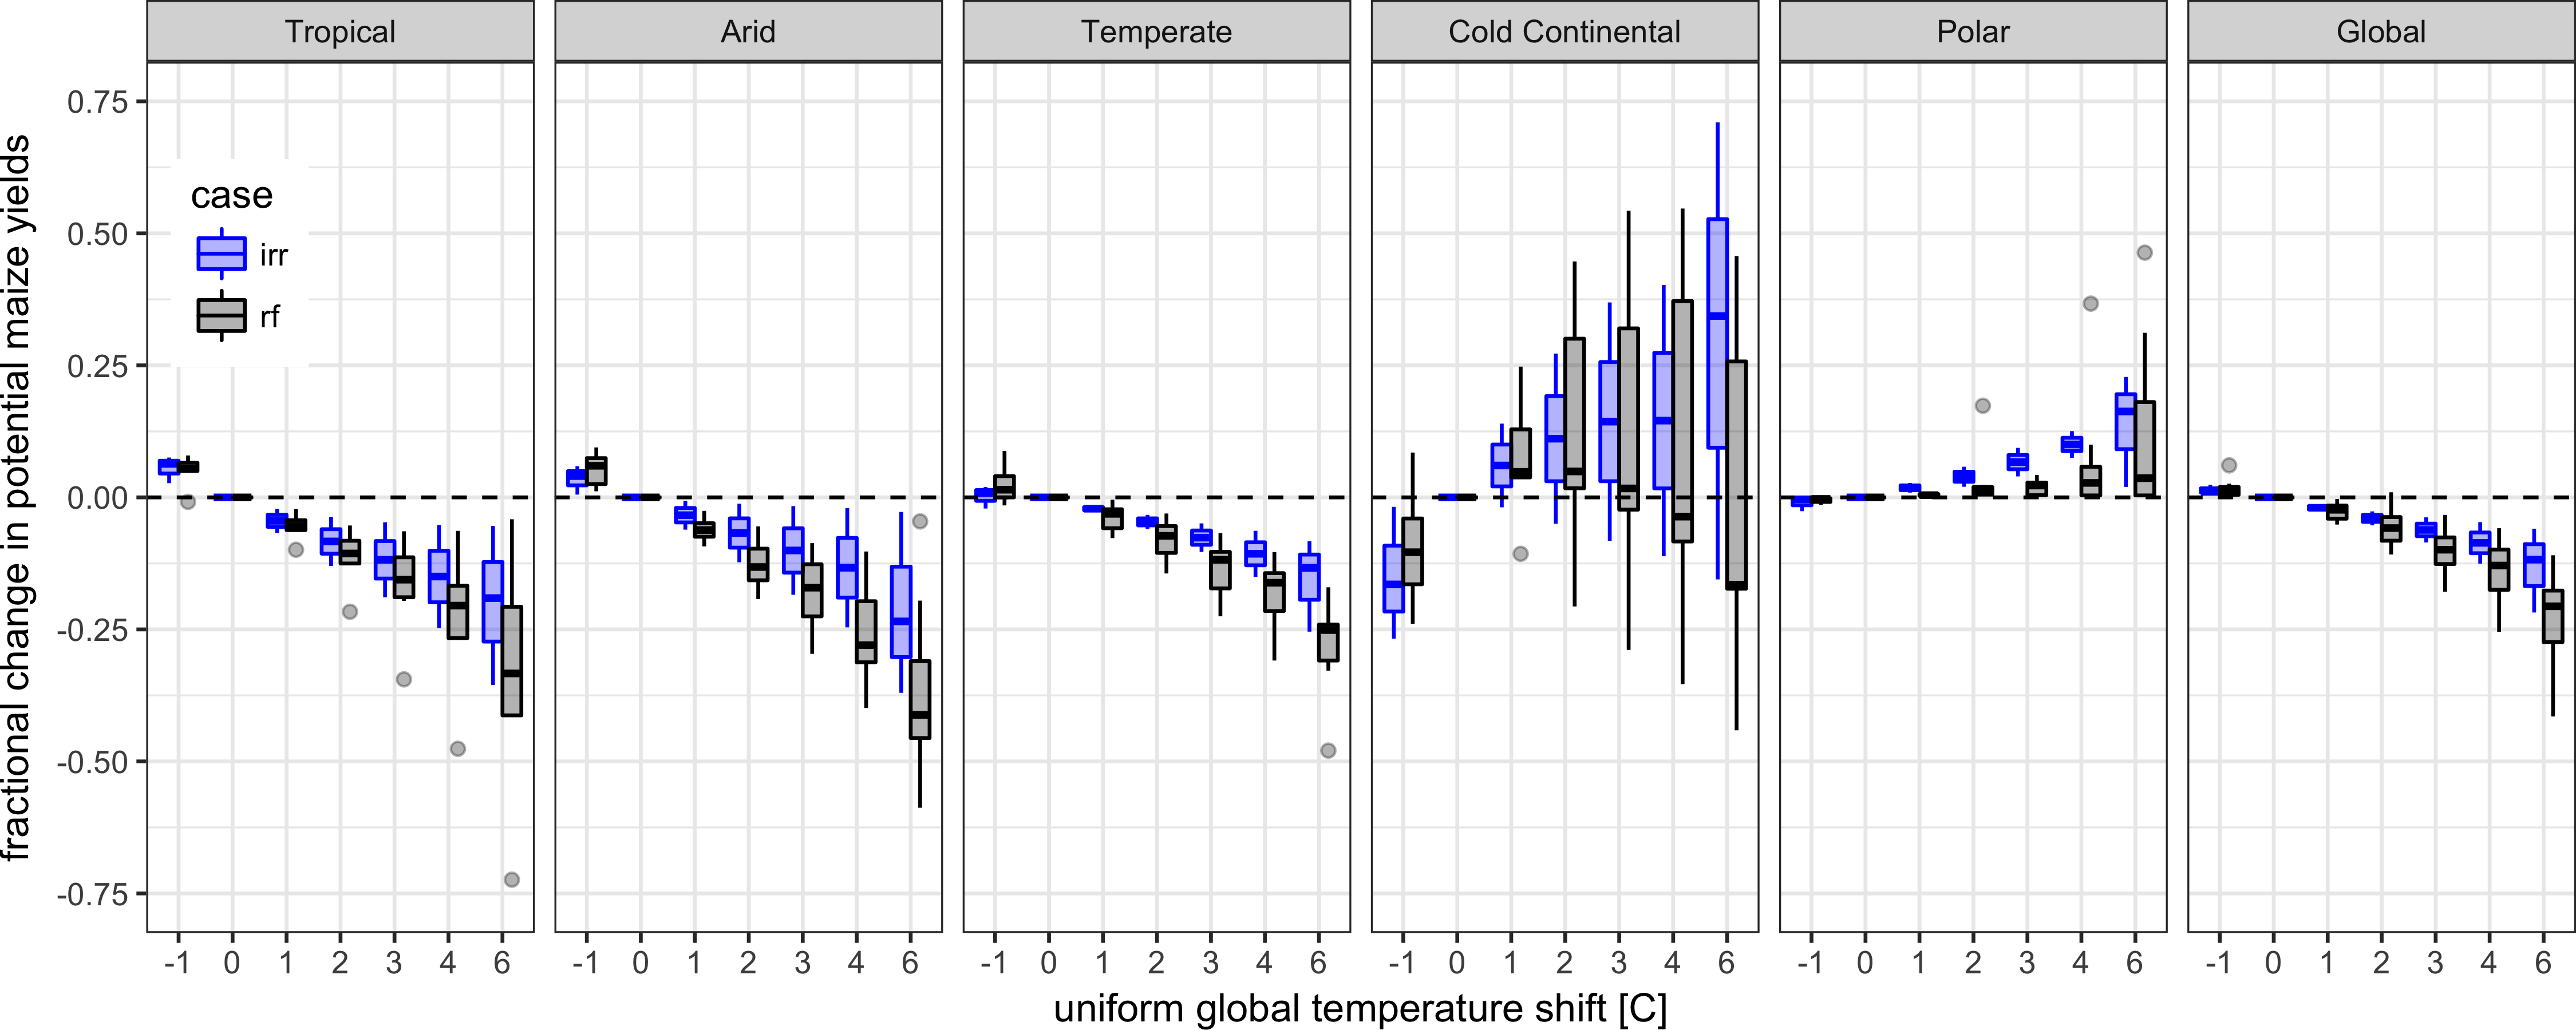
\includegraphics[width=\textwidth]{s_sim_KG_irr_all.png}\\
\caption{Irrigated maize has similar inter model variance as the baseline rain-fed case, but, shows greater resilience to temperature increases (reduced yield losses), especially in arid regions. All other covariates are held constant.}
\label{fig:KGirr_all}
\end{figure}

\begin{figure}[h!]
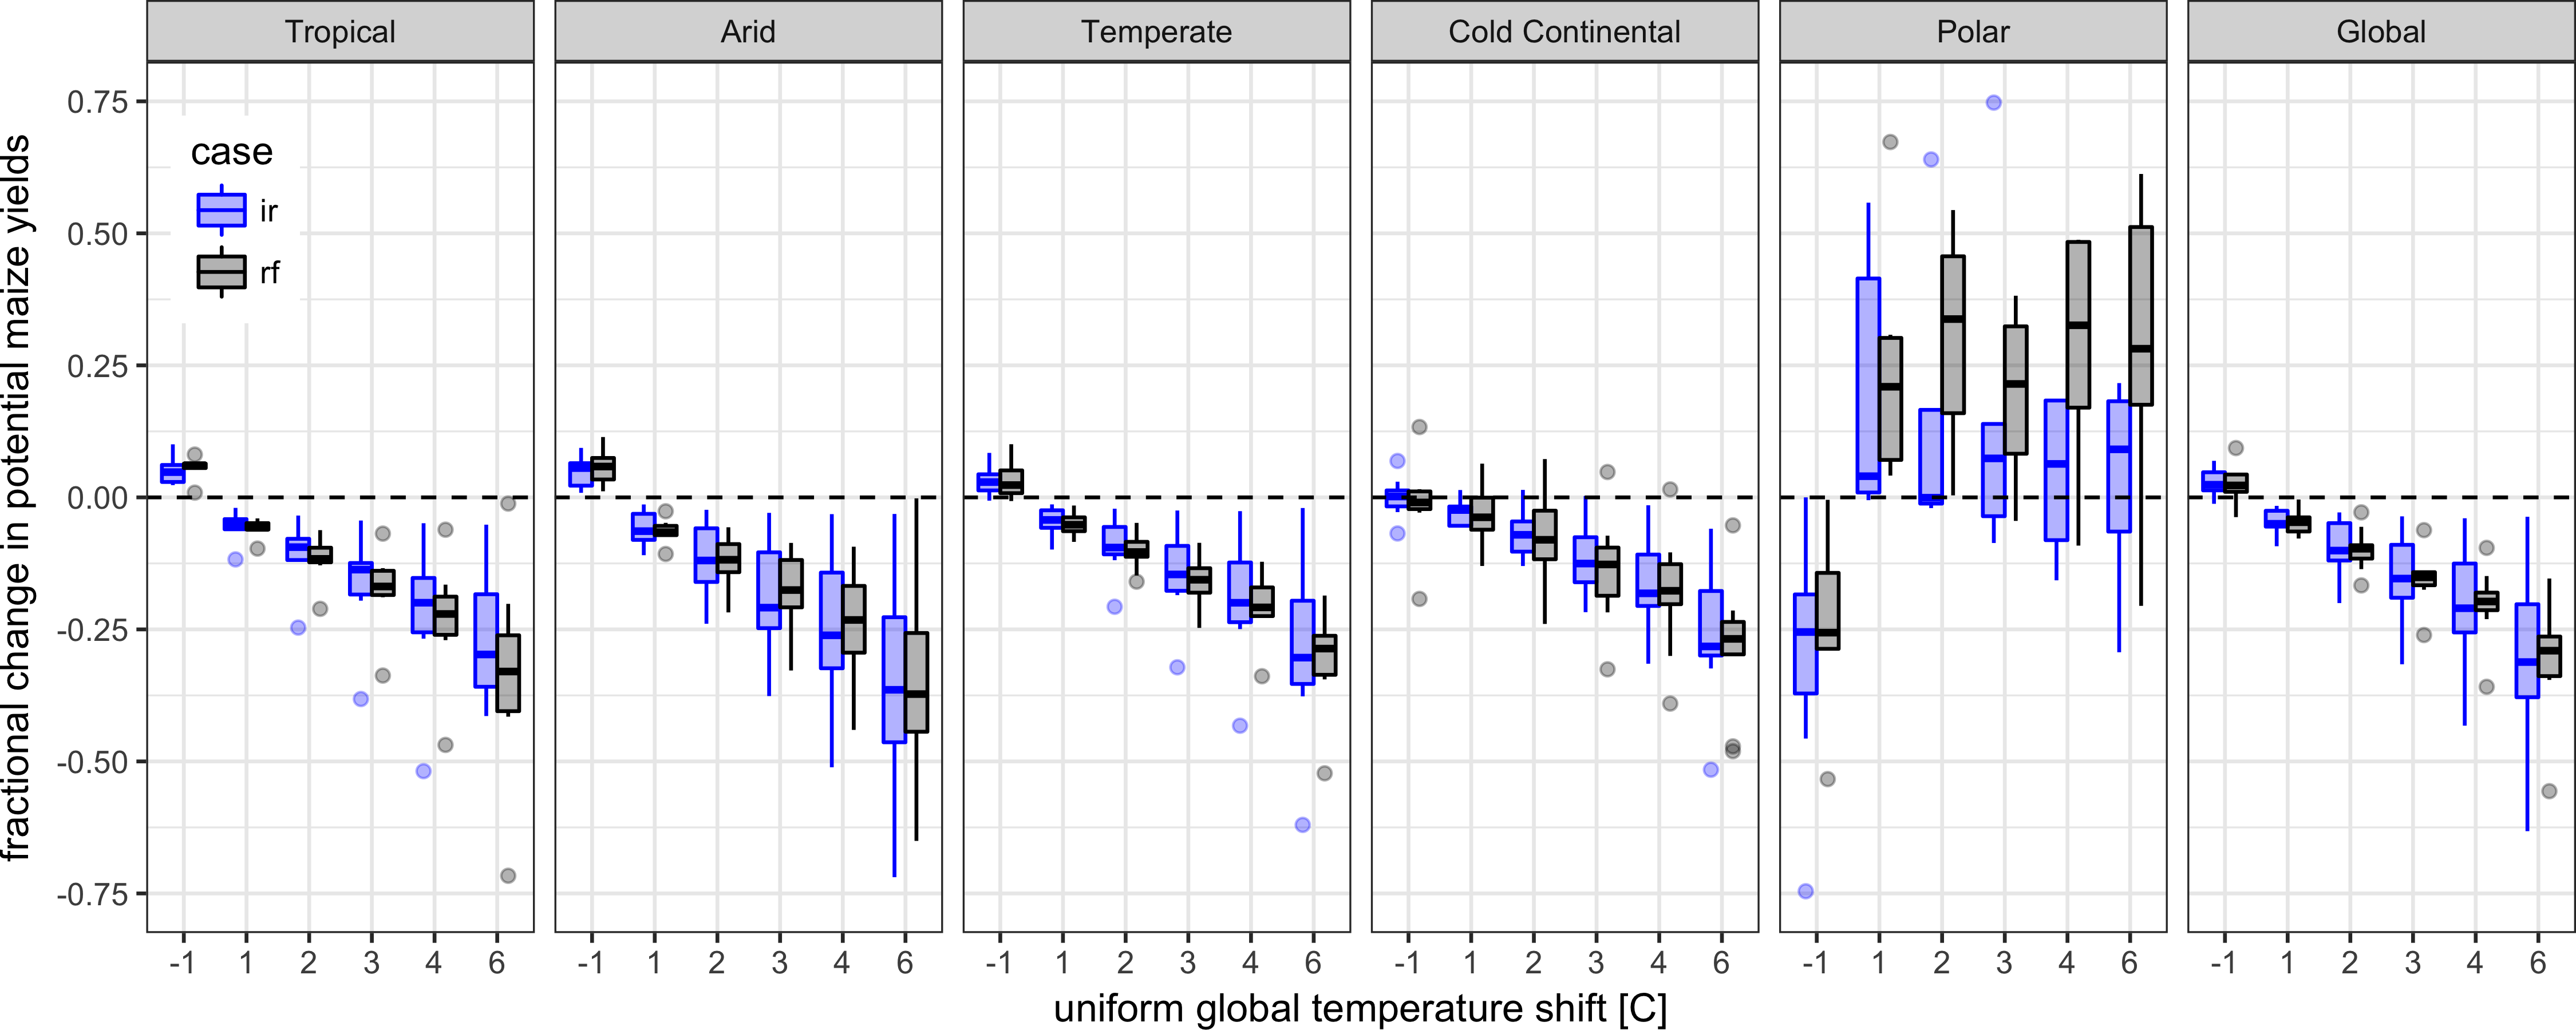
\includegraphics[width=\textwidth]{s_maize_sim_CG_area_weight.png}\\
\caption{Same figure as above but weighted by actual cultivation area in the real world. Due to difference in cultivation area, irrigated maize is more sensitive to increased temperature on currently cultivated area. All other covariates are held constant. PROMET and JULES not shown.}
\label{fig:KGirr_currentcult}
\end{figure}

\begin{figure}[h!]
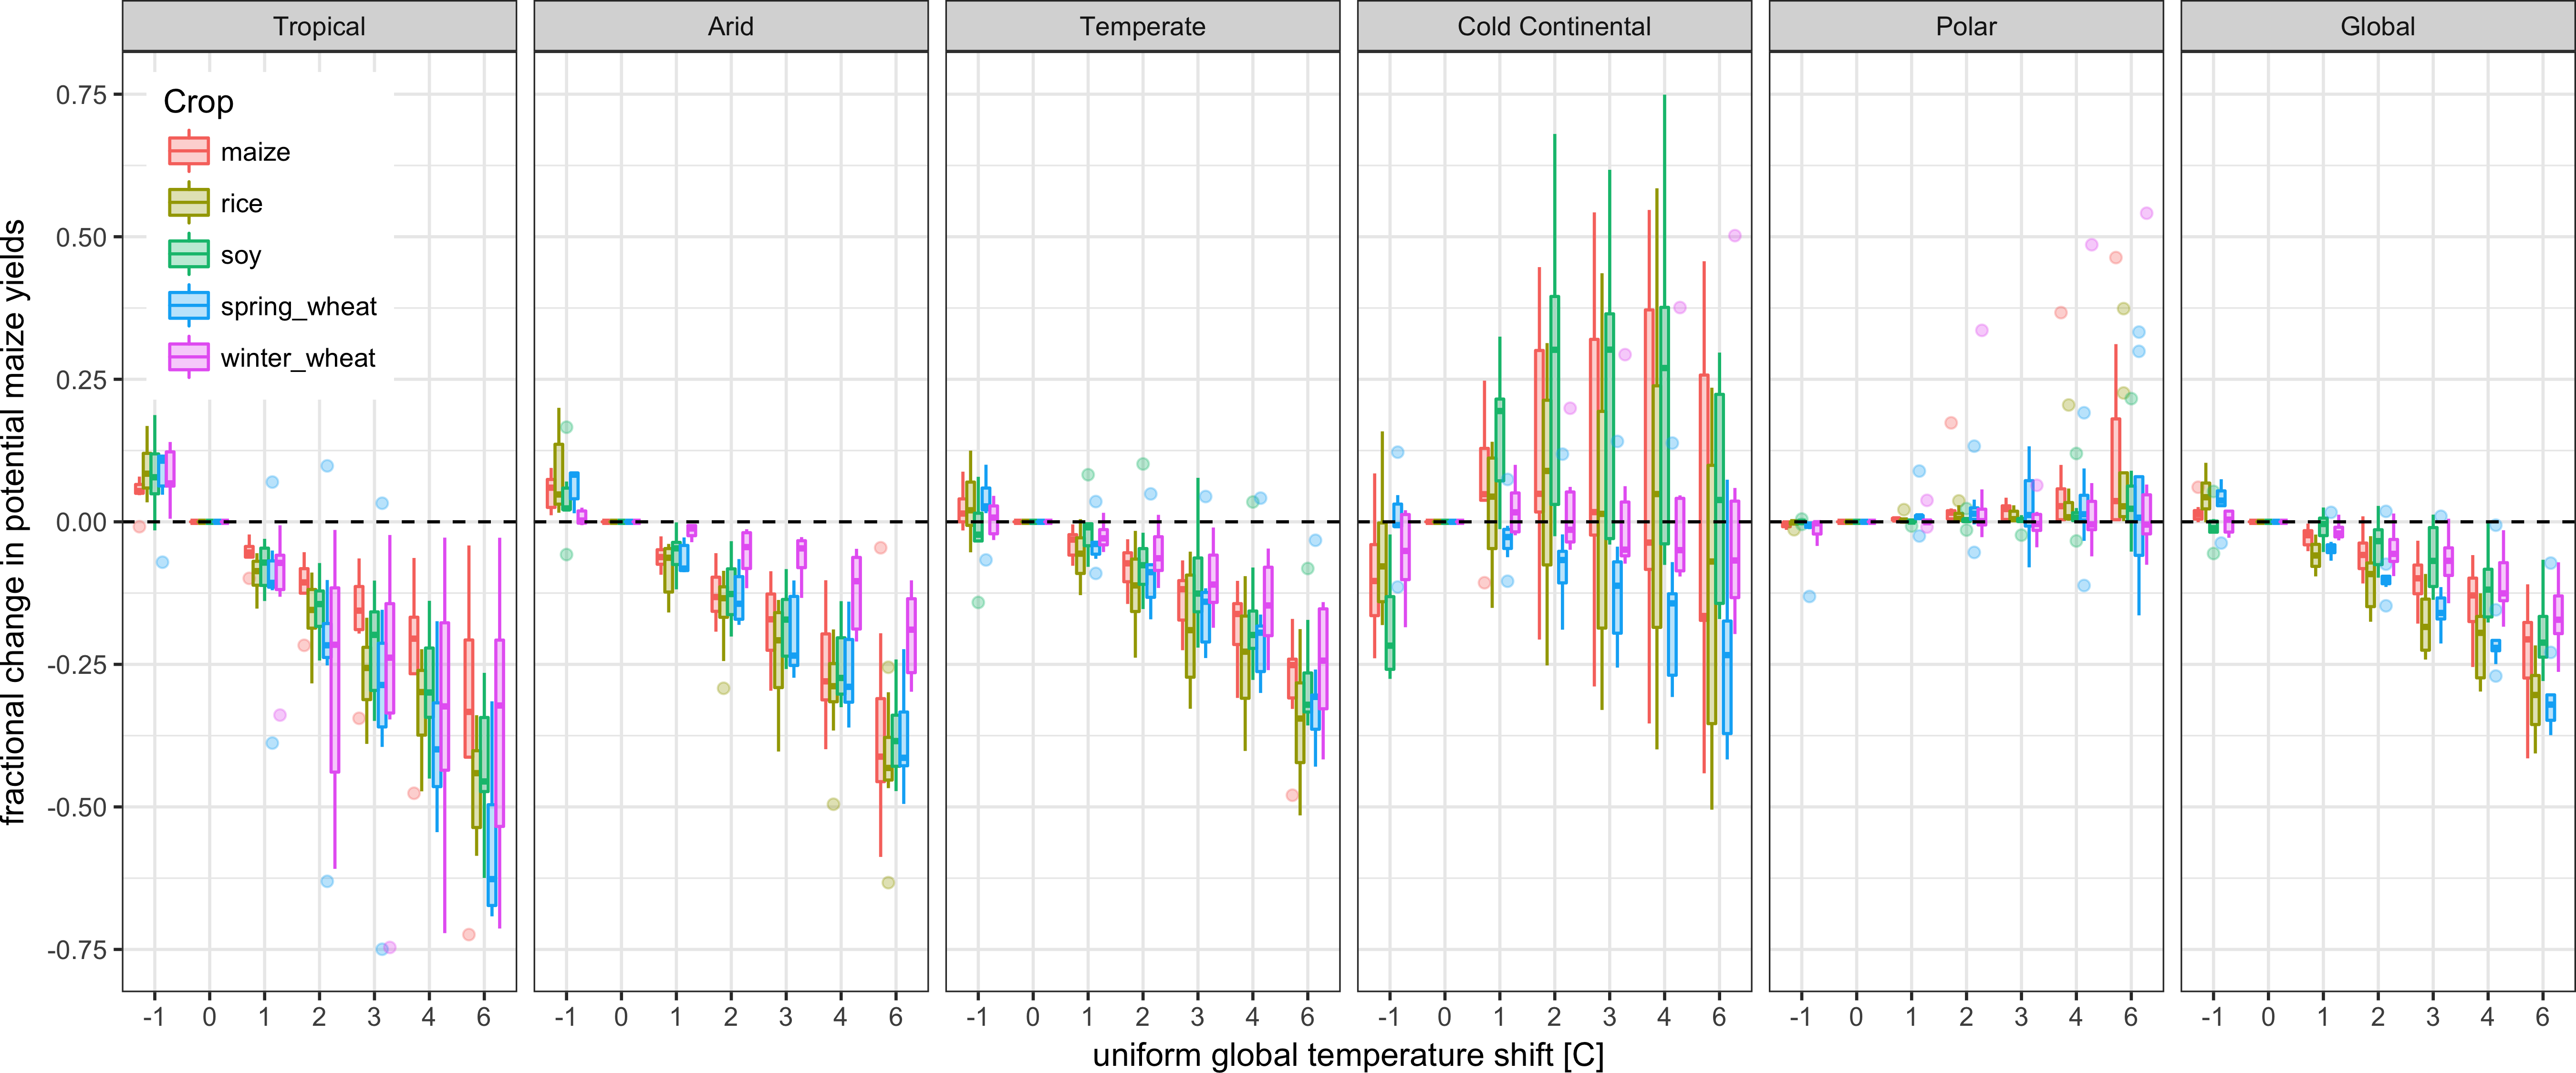
\includegraphics[width=\textwidth]{s_sim_KG_crops_all.png}\\
\caption{In cold continental regions, soy yields generally increase with warming and spring wheat yields decrease; the other crops are indeterminate across models. All other covariates are held constant.}
\label{fig:KGcrops_all}
\end{figure}

\begin{figure}[h!]
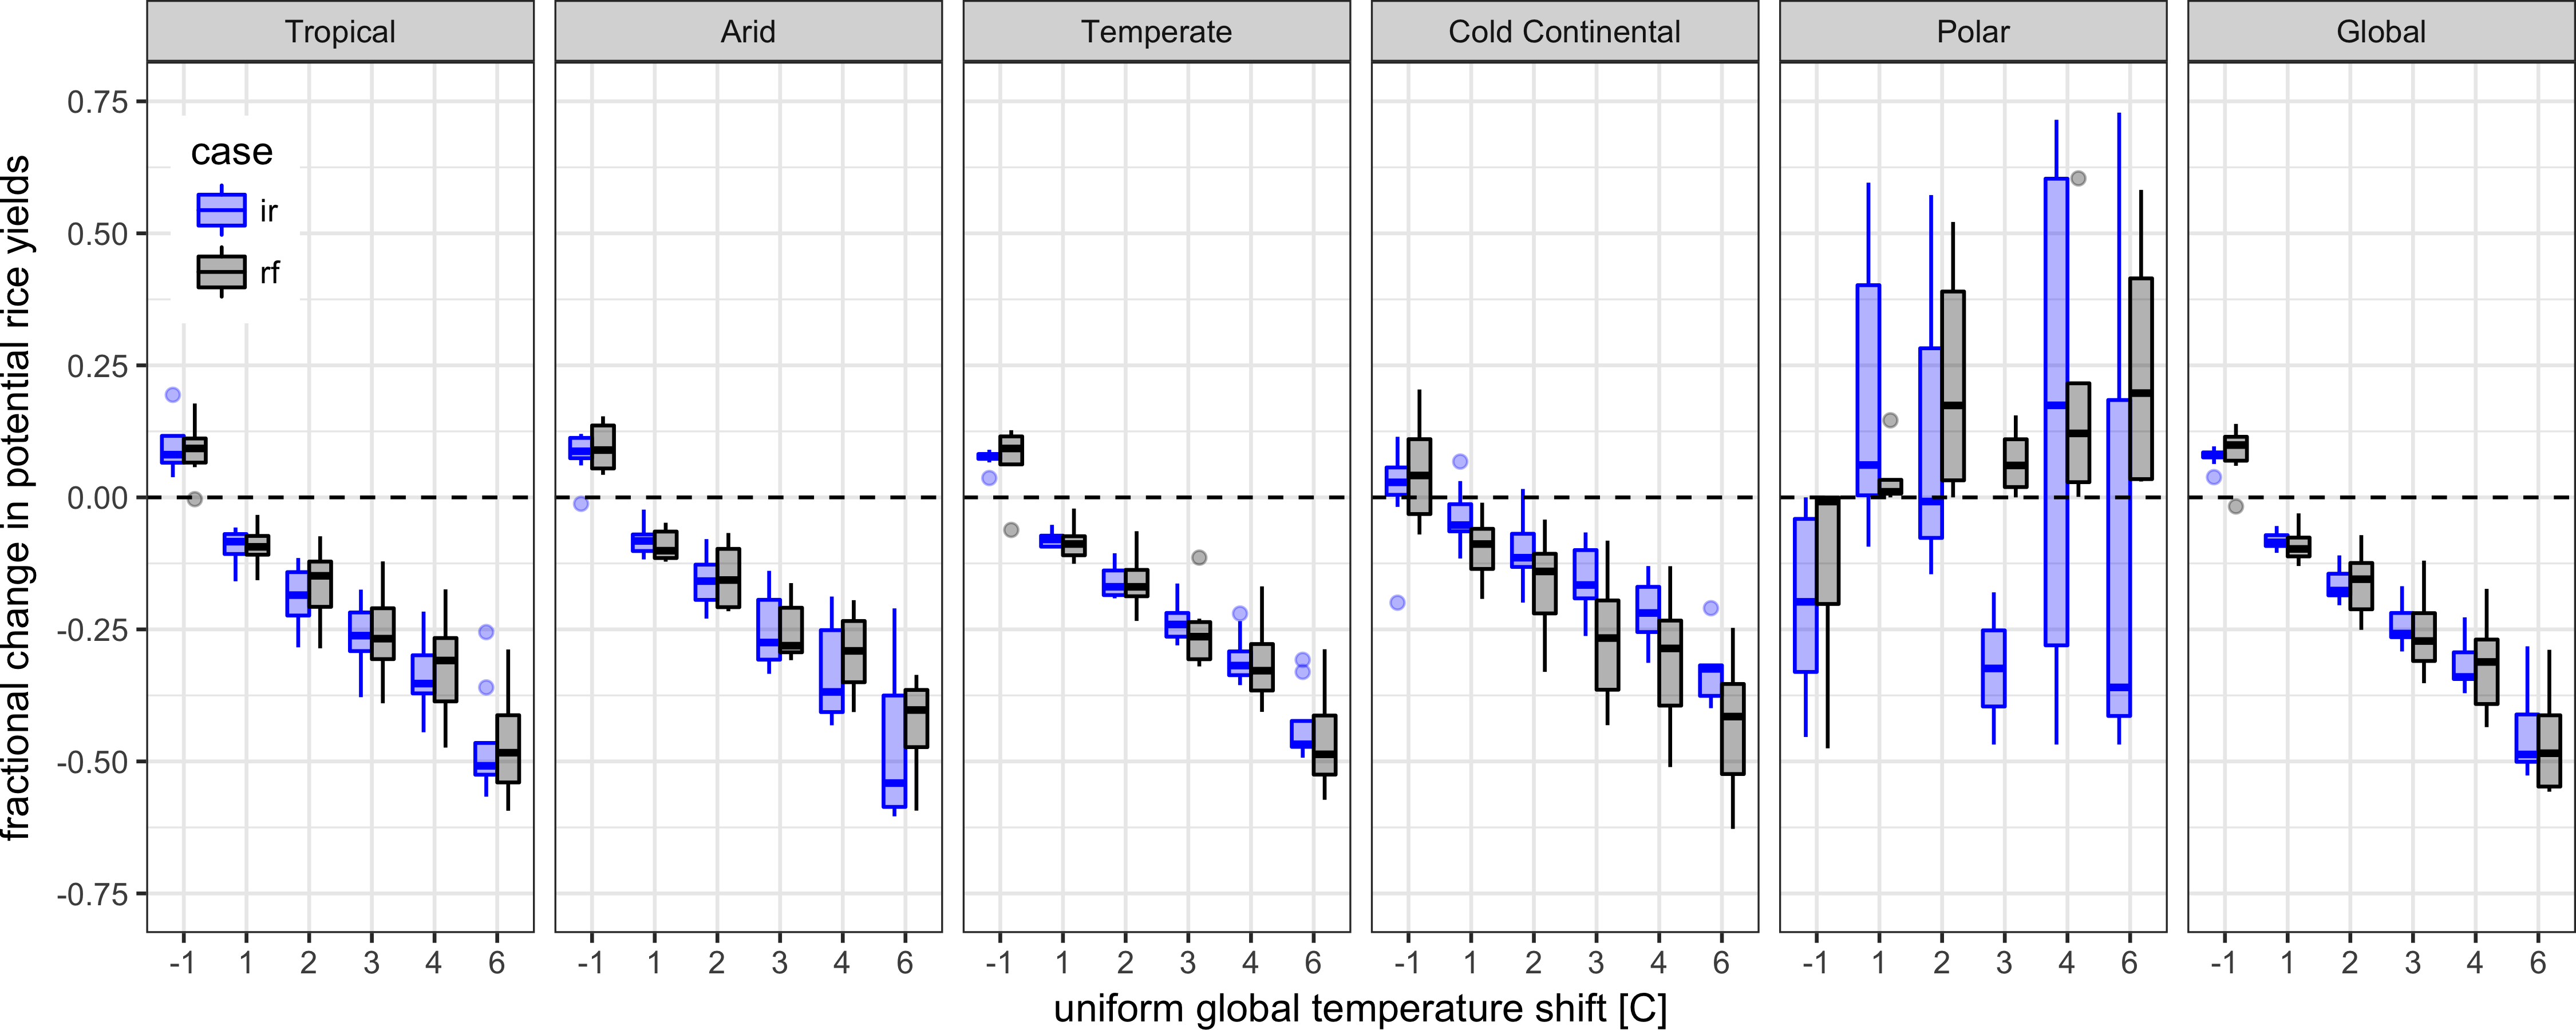
\includegraphics[width=\textwidth]{s_rice_sim_CG_area_weight.png}\\
\caption{Fractional change in rice production over currently cultivated areas for rain fed and irrigated rice. All other covariates are held constant. PROMET and JULES not shown. In contrast to maize, irrigated rice is not uniformly more severely impacted at higher temperatures.}
\label{fig:rice_currentcult}
\end{figure}

\begin{figure}[h!]
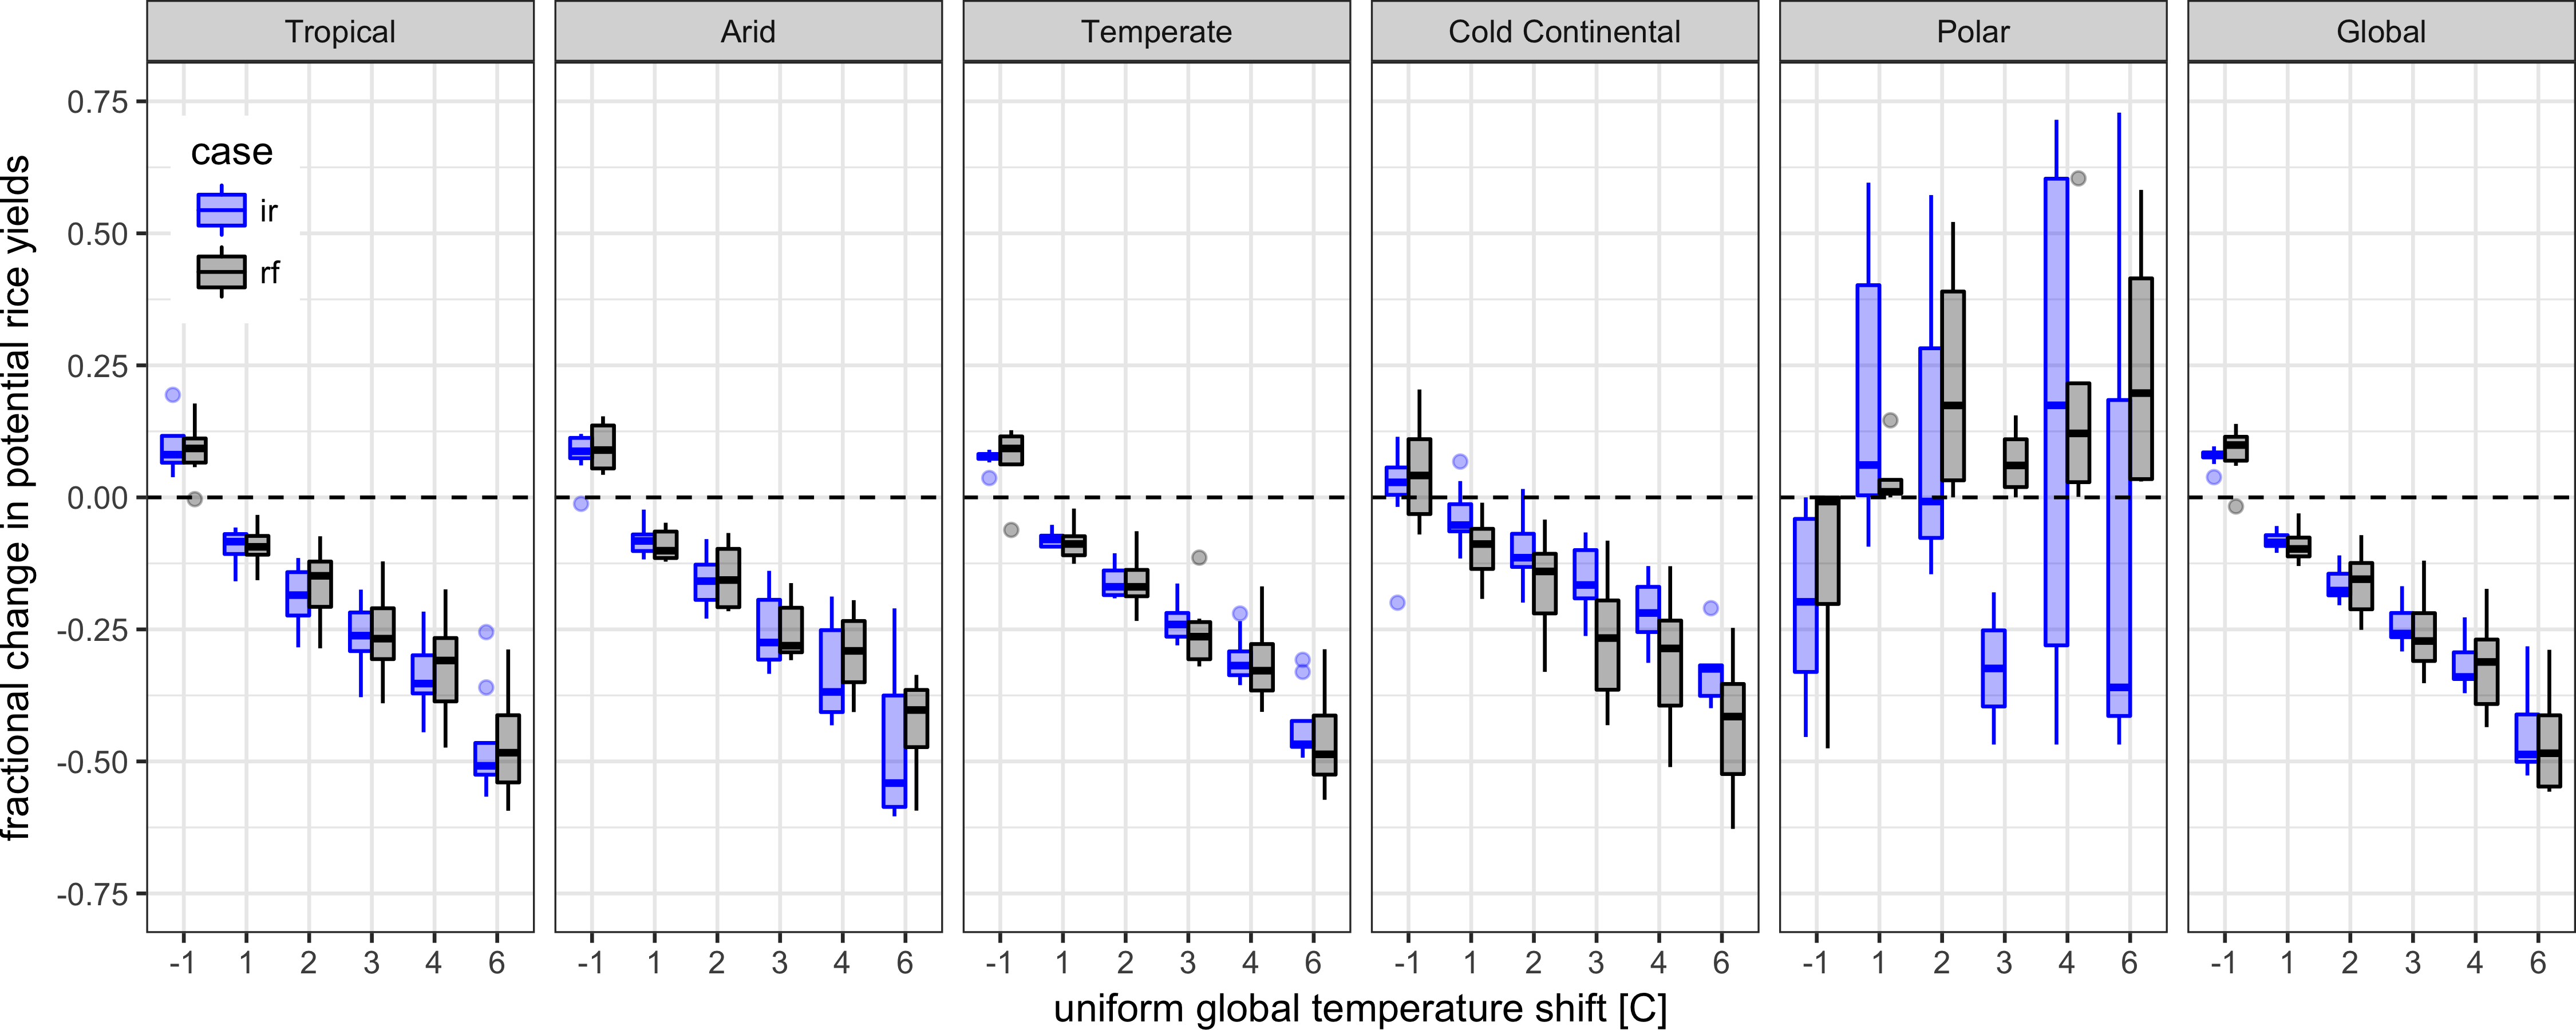
\includegraphics[width=\textwidth]{s_rice_sim_CG_area_weight.png}\\
\caption{Fractional change in soy production over currently cultivated areas for rain-fed and irrigated rice. All other covariates are held constant. PROMET and JULES not shown. In contrast to maize, irrigated soy is not uniformly more severely impacted at higher temperatures.}
\label{fig:soy_currentcult}
\end{figure}

\begin{figure}[h!]
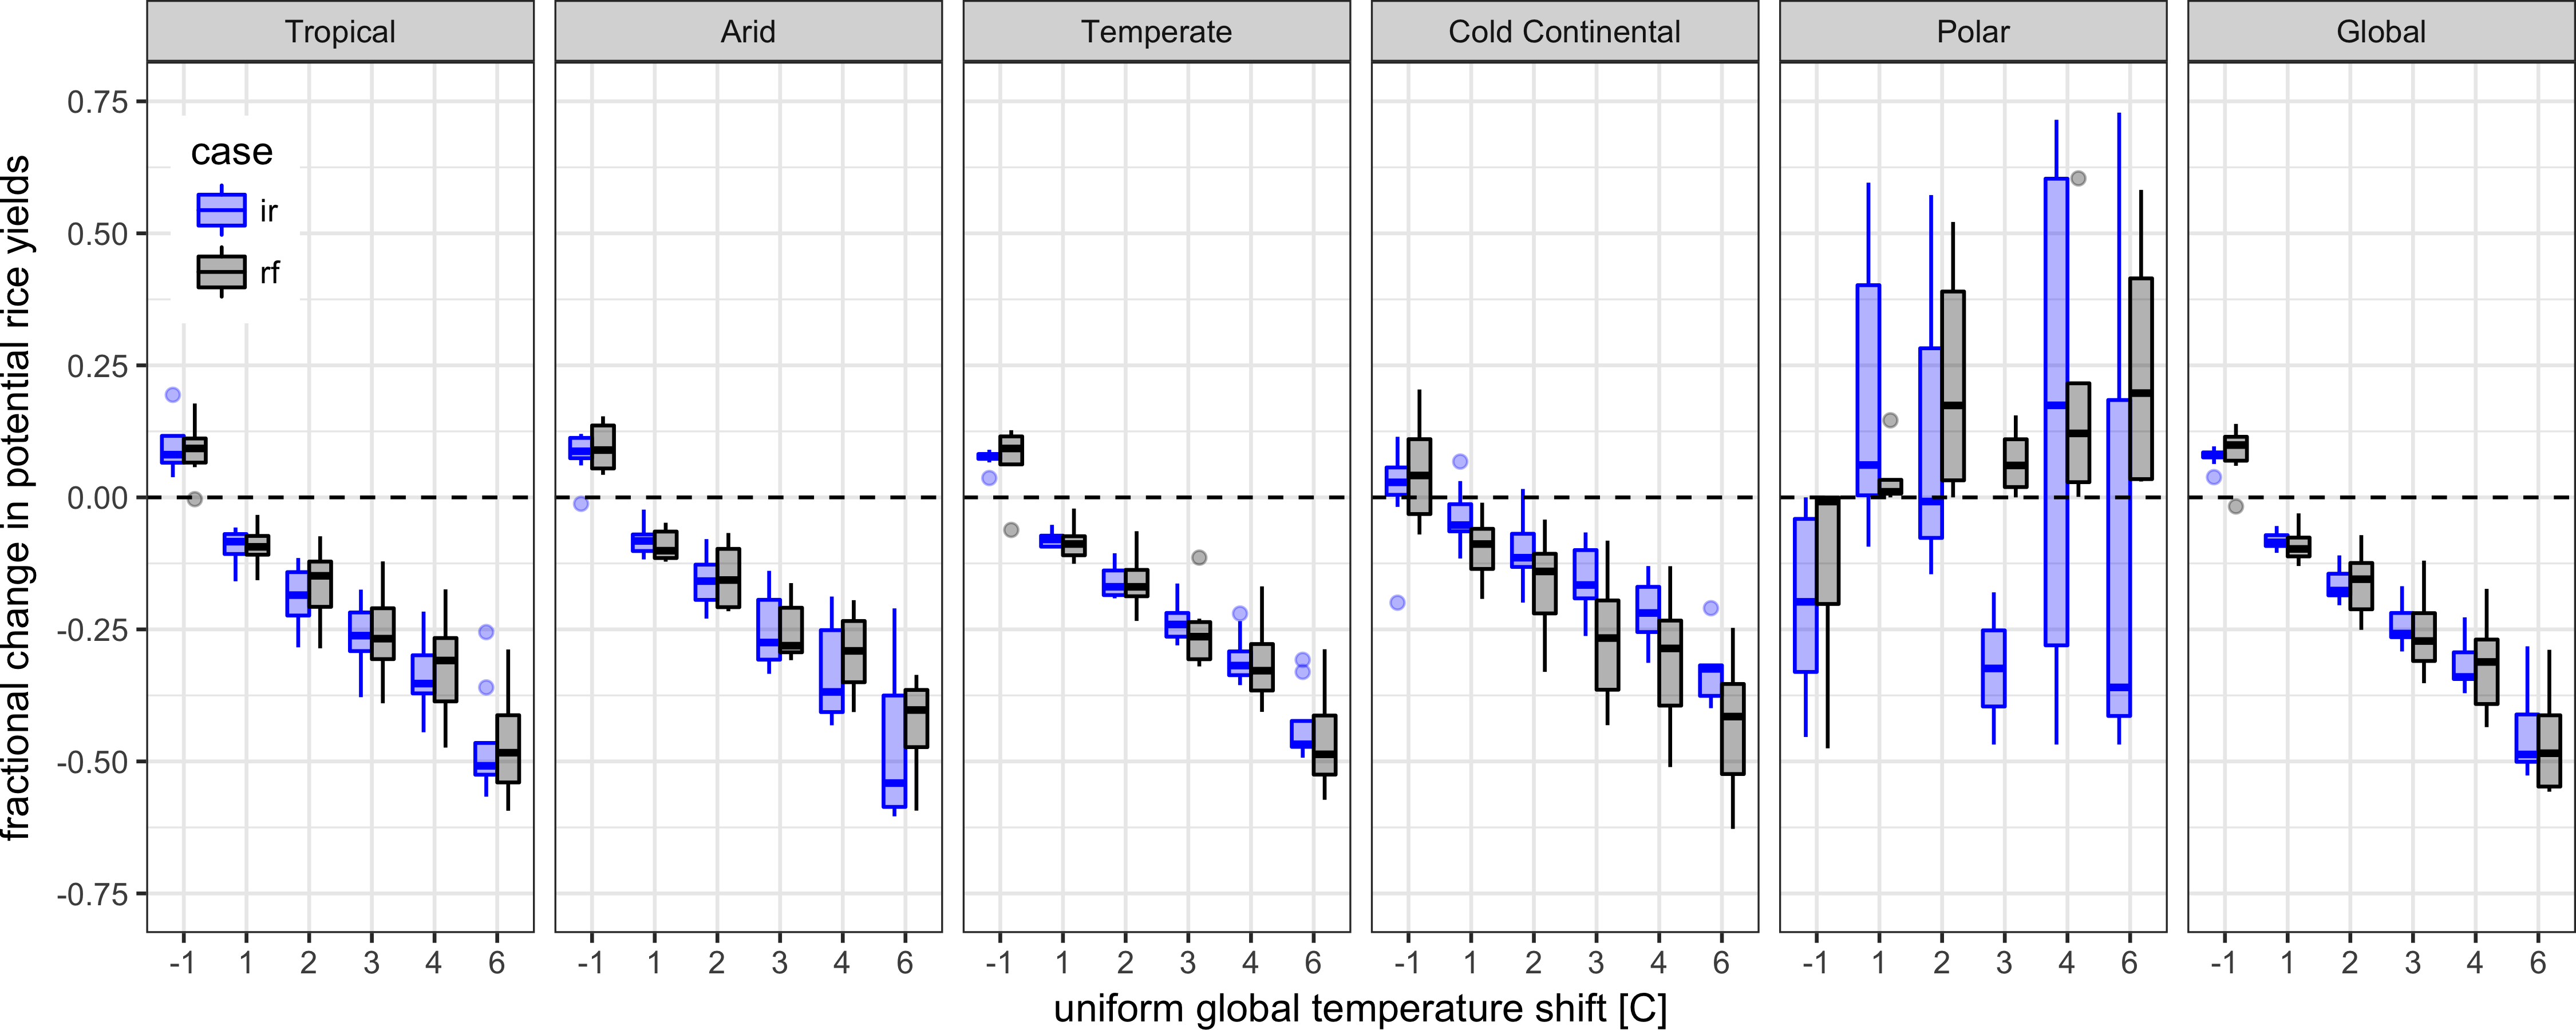
\includegraphics[width=\textwidth]{s_rice_sim_CG_area_weight.png}\\
\caption{Fractional change in winter wheat production over currently cultivated areas for rain fed and irrigated rice. All other covariates are held constant. PROMET and JULES not shown.}
\label{fig:winter_wheat_currentcult}
\end{figure}

\begin{figure}[h!]
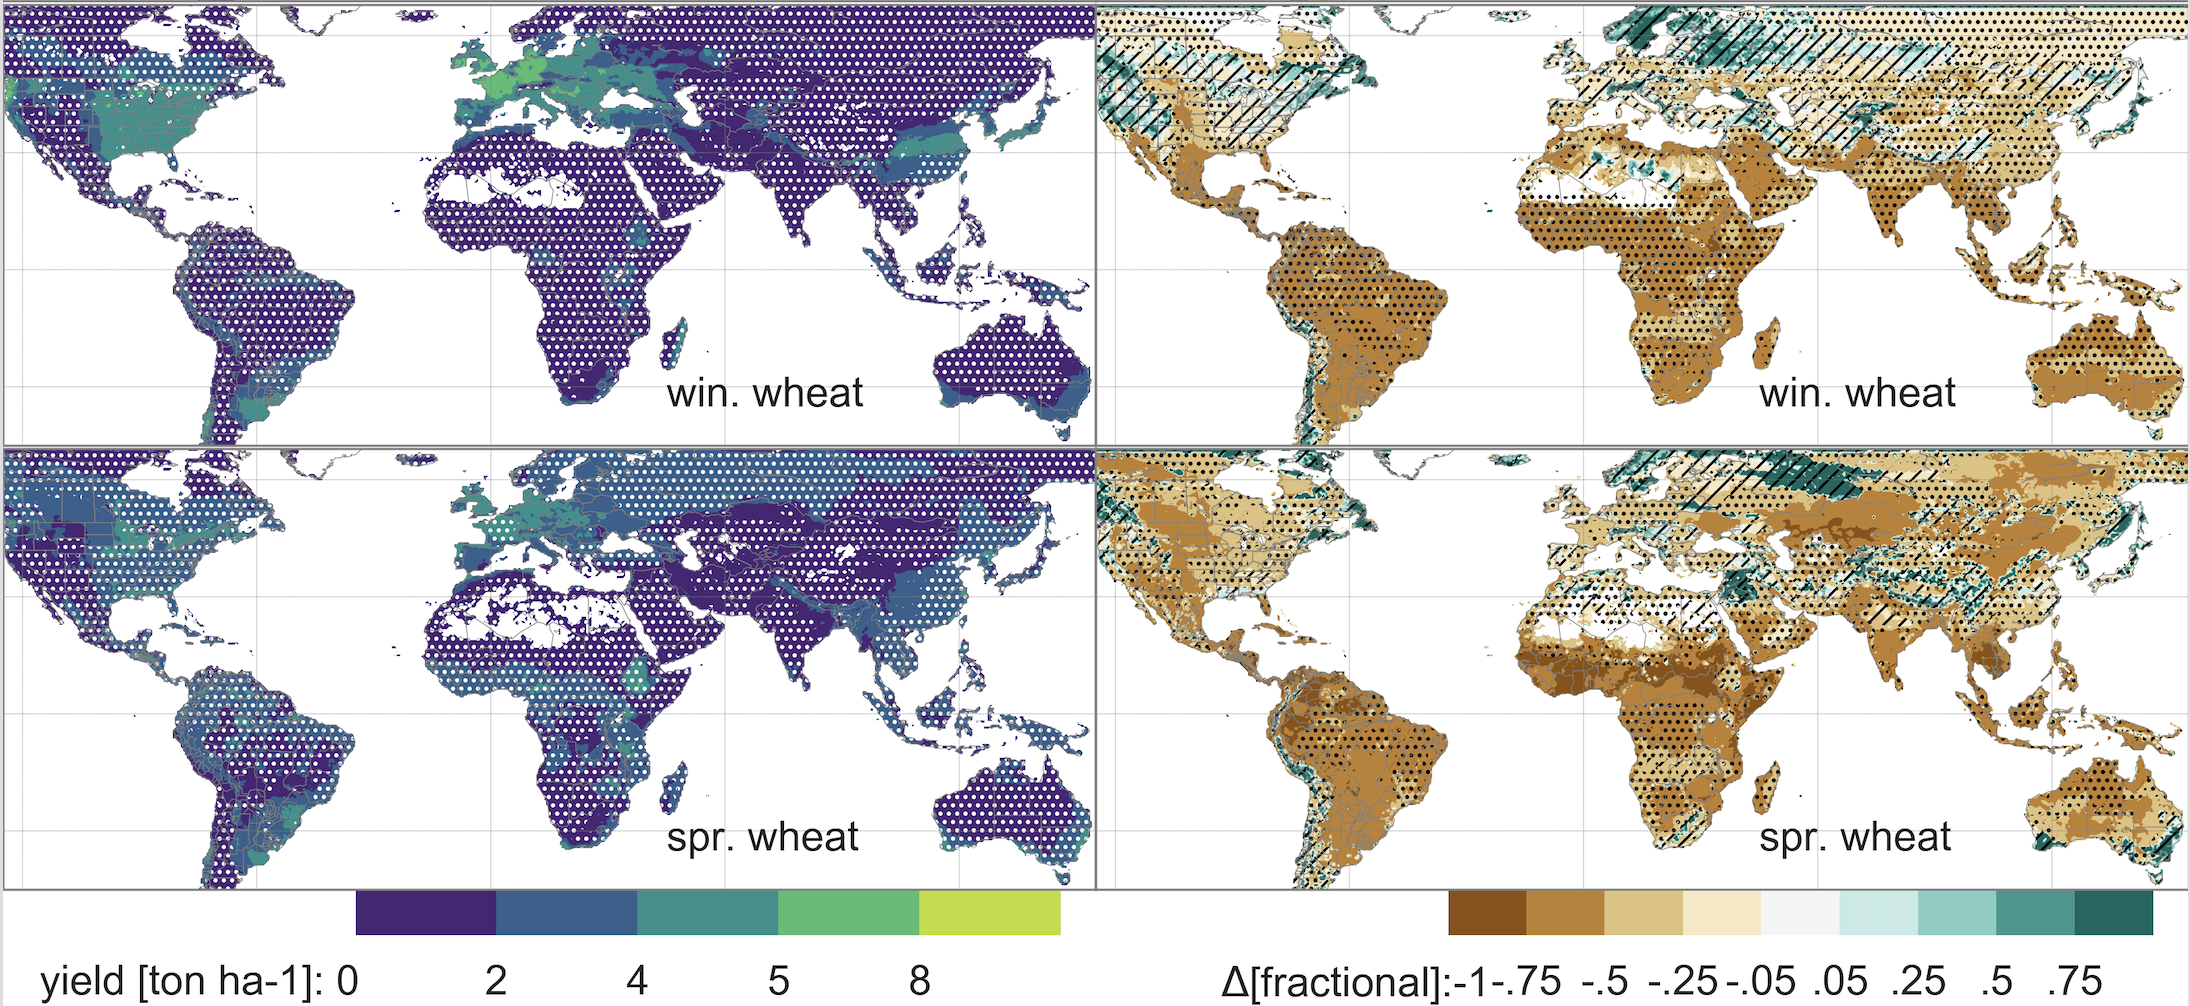
\includegraphics[width=\textwidth]{s_wheat_baseline.png}\\
\caption{Illustration of the spatial pattern of potential yields and potential yield changes in the GGCMI Phase II ensemble, for three major crops. Left column (a) shows multi-model mean climatological yields for the baseline scenario for (top--bottom) for rain-fed wheat. White stippling indicates areas where these crops are not currently cultivated. Absence of cultivation aligns well with the lowest yield contour (0-2 ton ha$^{-1}$). Right column (b) shows the multi-model mean fractional yield change in the extreme T + 4 $^{\circ}$C scenario (with other inputs at baseline values). Areas without hatching or stippling are those where confidence in projections is high: the multi-model mean fractional change exceeds two standard deviations of the ensemble. ($\Delta > 2\sigma$). Hatching indicates areas of low confidence ($\Delta < 1 \sigma$), and stippling areas of medium confidence ($1 \sigma < \Delta < 2 \sigma$). Crop model results in cold areas, where yield impacts are on average positive, also have the highest uncertainty. Wheat is also somewhat exceptional in that  also less impact in temperature and arid regions. The more complicated phenological development of winter wheat when compared to other crops is a potential source of the higher level of model disagreement.}
\label{fig:wheatbaseline}
\end{figure}

\clearpage
\section{Emulator fits and performance}
Additional emulator performance figures for reference. PROMET and JULES are shown because these two models are the most-difficult to emulate.

\begin{figure}[h!]
\centering
\begin{minipage}{.45\textwidth}
    \centering
    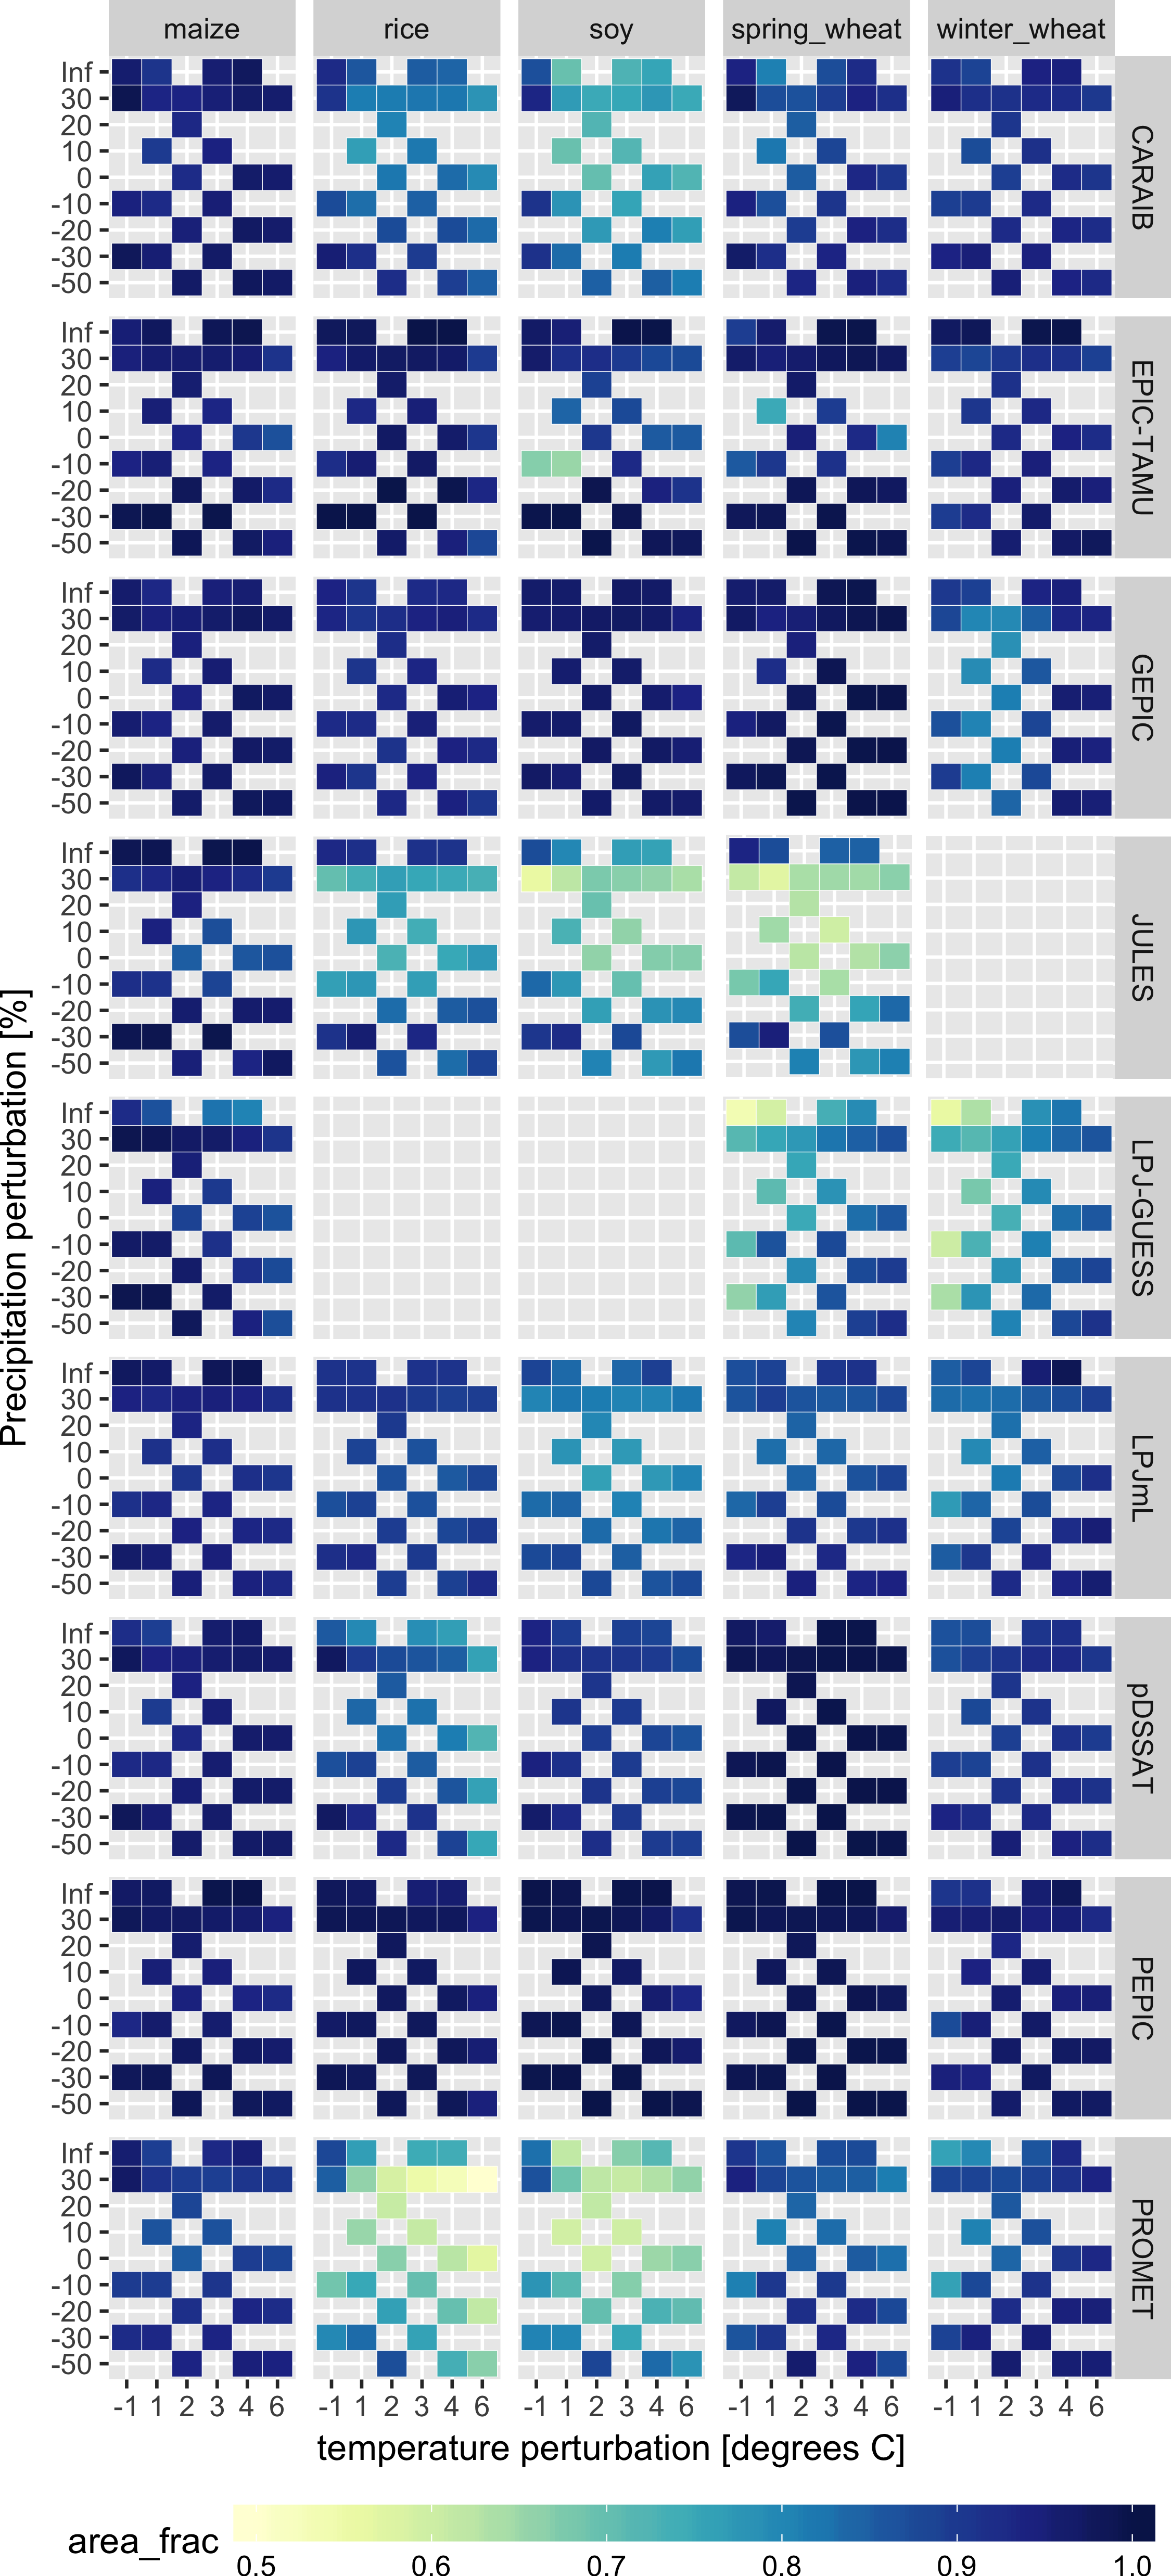
\includegraphics[width=\textwidth]{s_error_360_total.png}\\
    \caption{The fraction of grid cells with normalized emulation error less than 1 for the CO$_2$=360 ppm and 200 kg~N ha$^{-1}$ yr$^{-1}$ case for the temperature and precipitation perturbations scenarios provided by all 9 models included in the emulator analysis. This is in contrast to the fraction of currently cultivated hectares shown in the C360 case in the manuscript and for the C810 case show in the supplemental material. The emulator is marginally more successful over currently cultivated areas than over all grid cells in general.}
    \label{fig:error360total}
\end{minipage}
\hspace{.05\linewidth}
\begin{minipage}{.45\textwidth}
    \centering
    \vspace{0pt}
    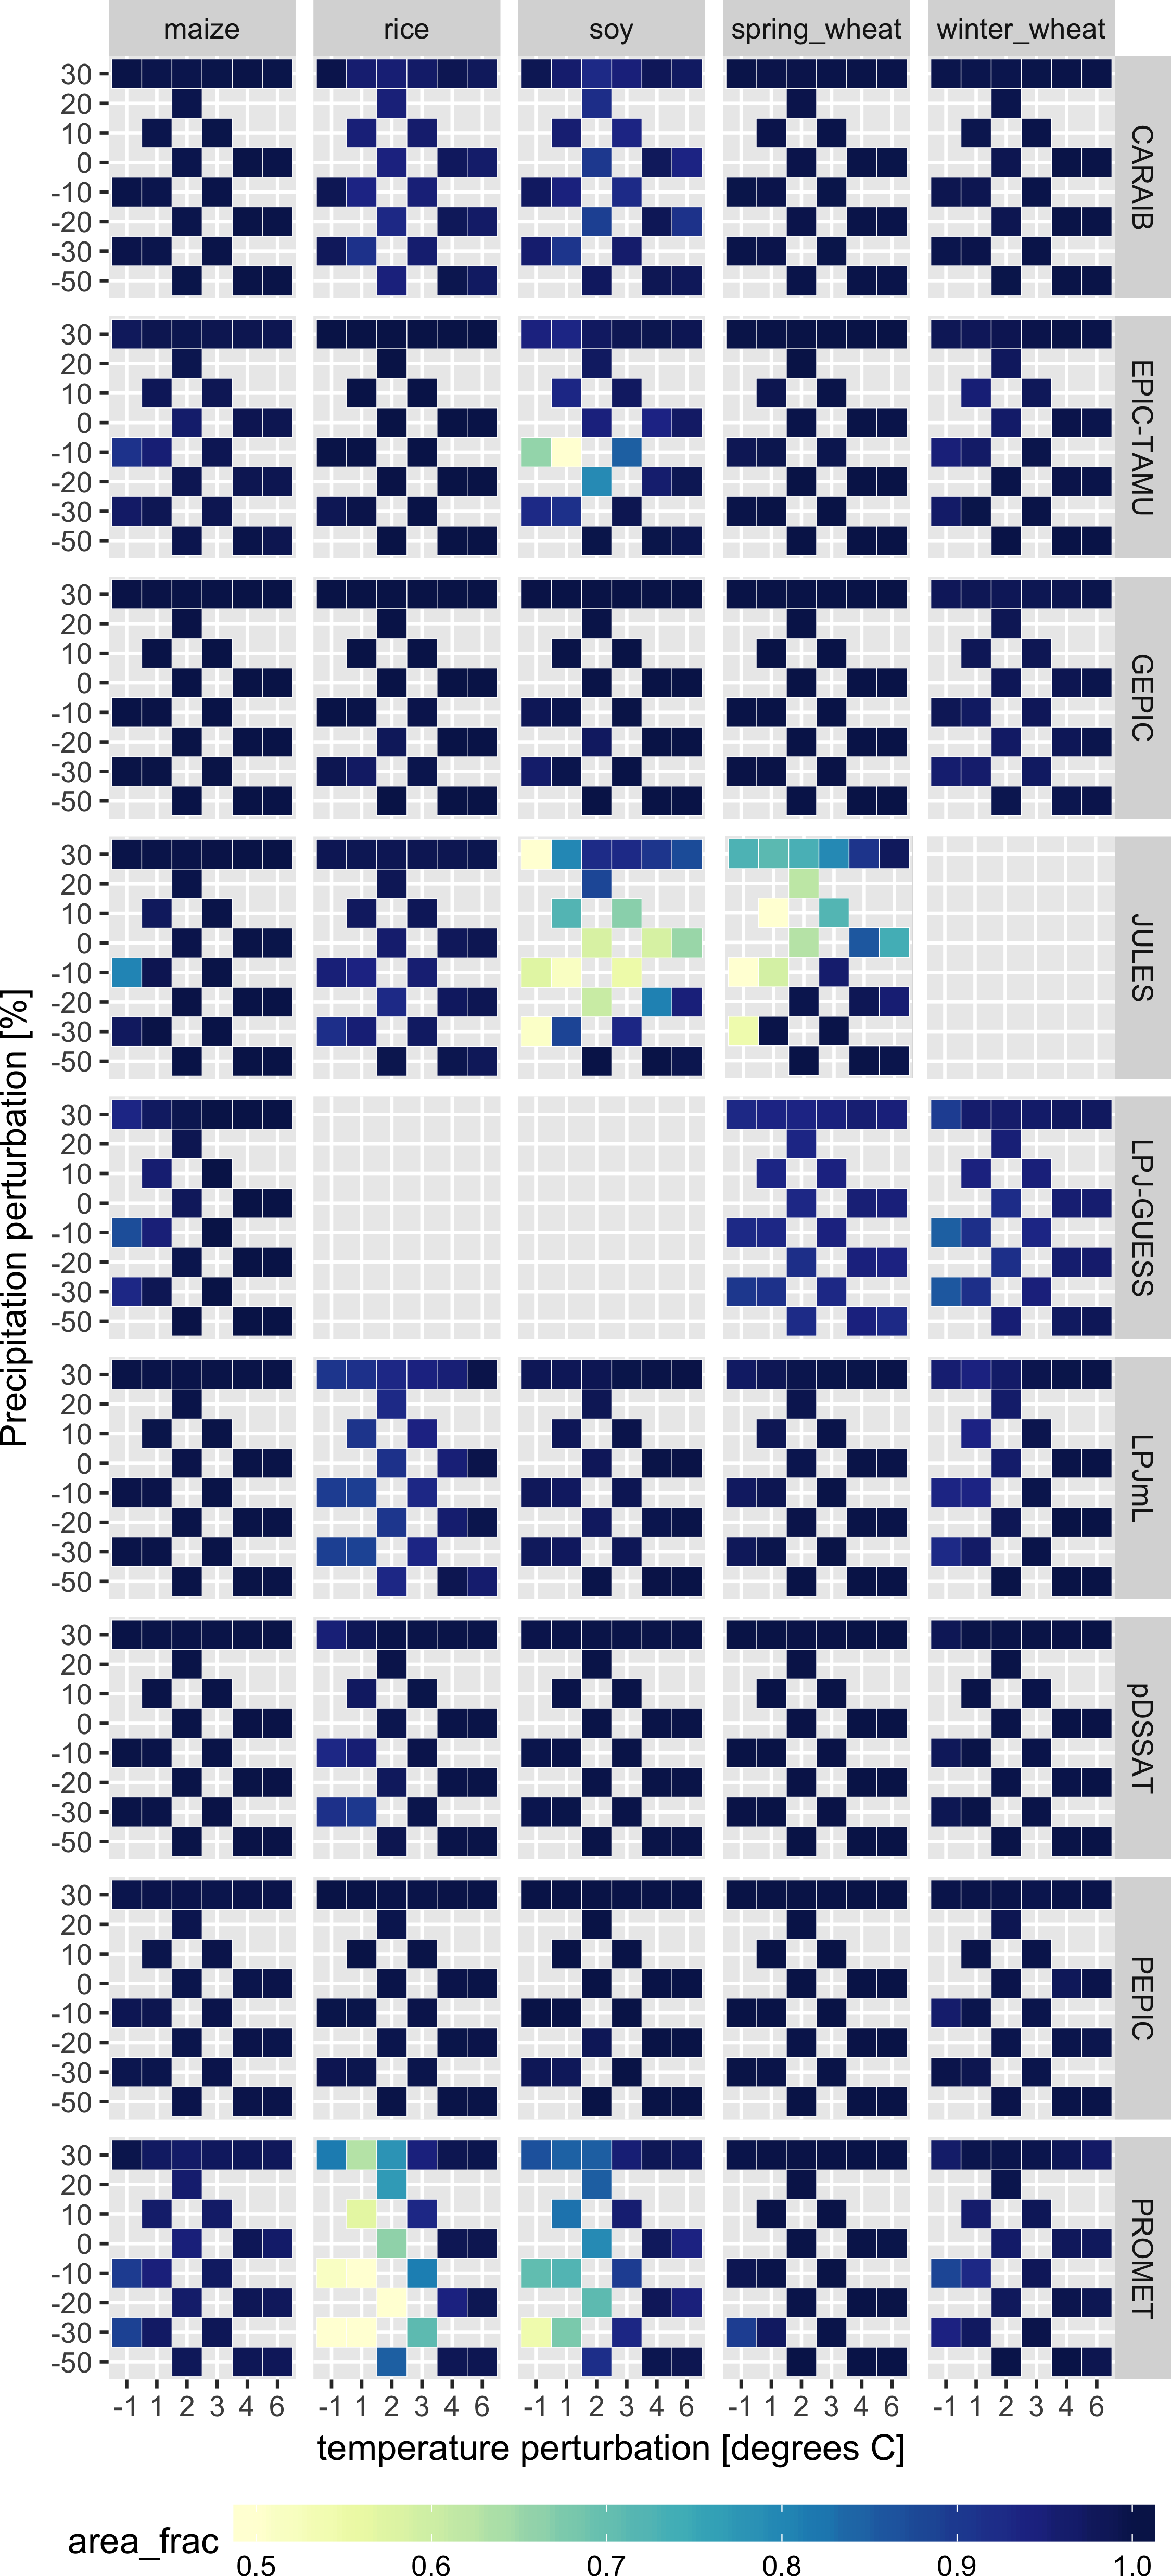
\includegraphics[width=\textwidth]{s_error_810.png}\\
    \caption{The fraction of currently cultivated hectares with normalized emulation error less than 1 (blue colors contours in Figure \ref{fig:error}) for the CO$_2$=810 ppm and 200 kg~N ha$^{-1}$ yr$^{-1}$ case for the temperature and precipitation perturbations scenarios provided by all 9 models included in the emulator analysis. See Equations \ref{eqn:error}, \ref{eqn:per_yield} for normalized error calculation. The yield response is generally easy to emulate over currently cultivated areas (dark blue and light blue).}
    \label{fig:error810}
\end{minipage}
\end{figure}

\begin{figure}[h!]
\centering
\begin{minipage}{.45\textwidth}
    \centering
    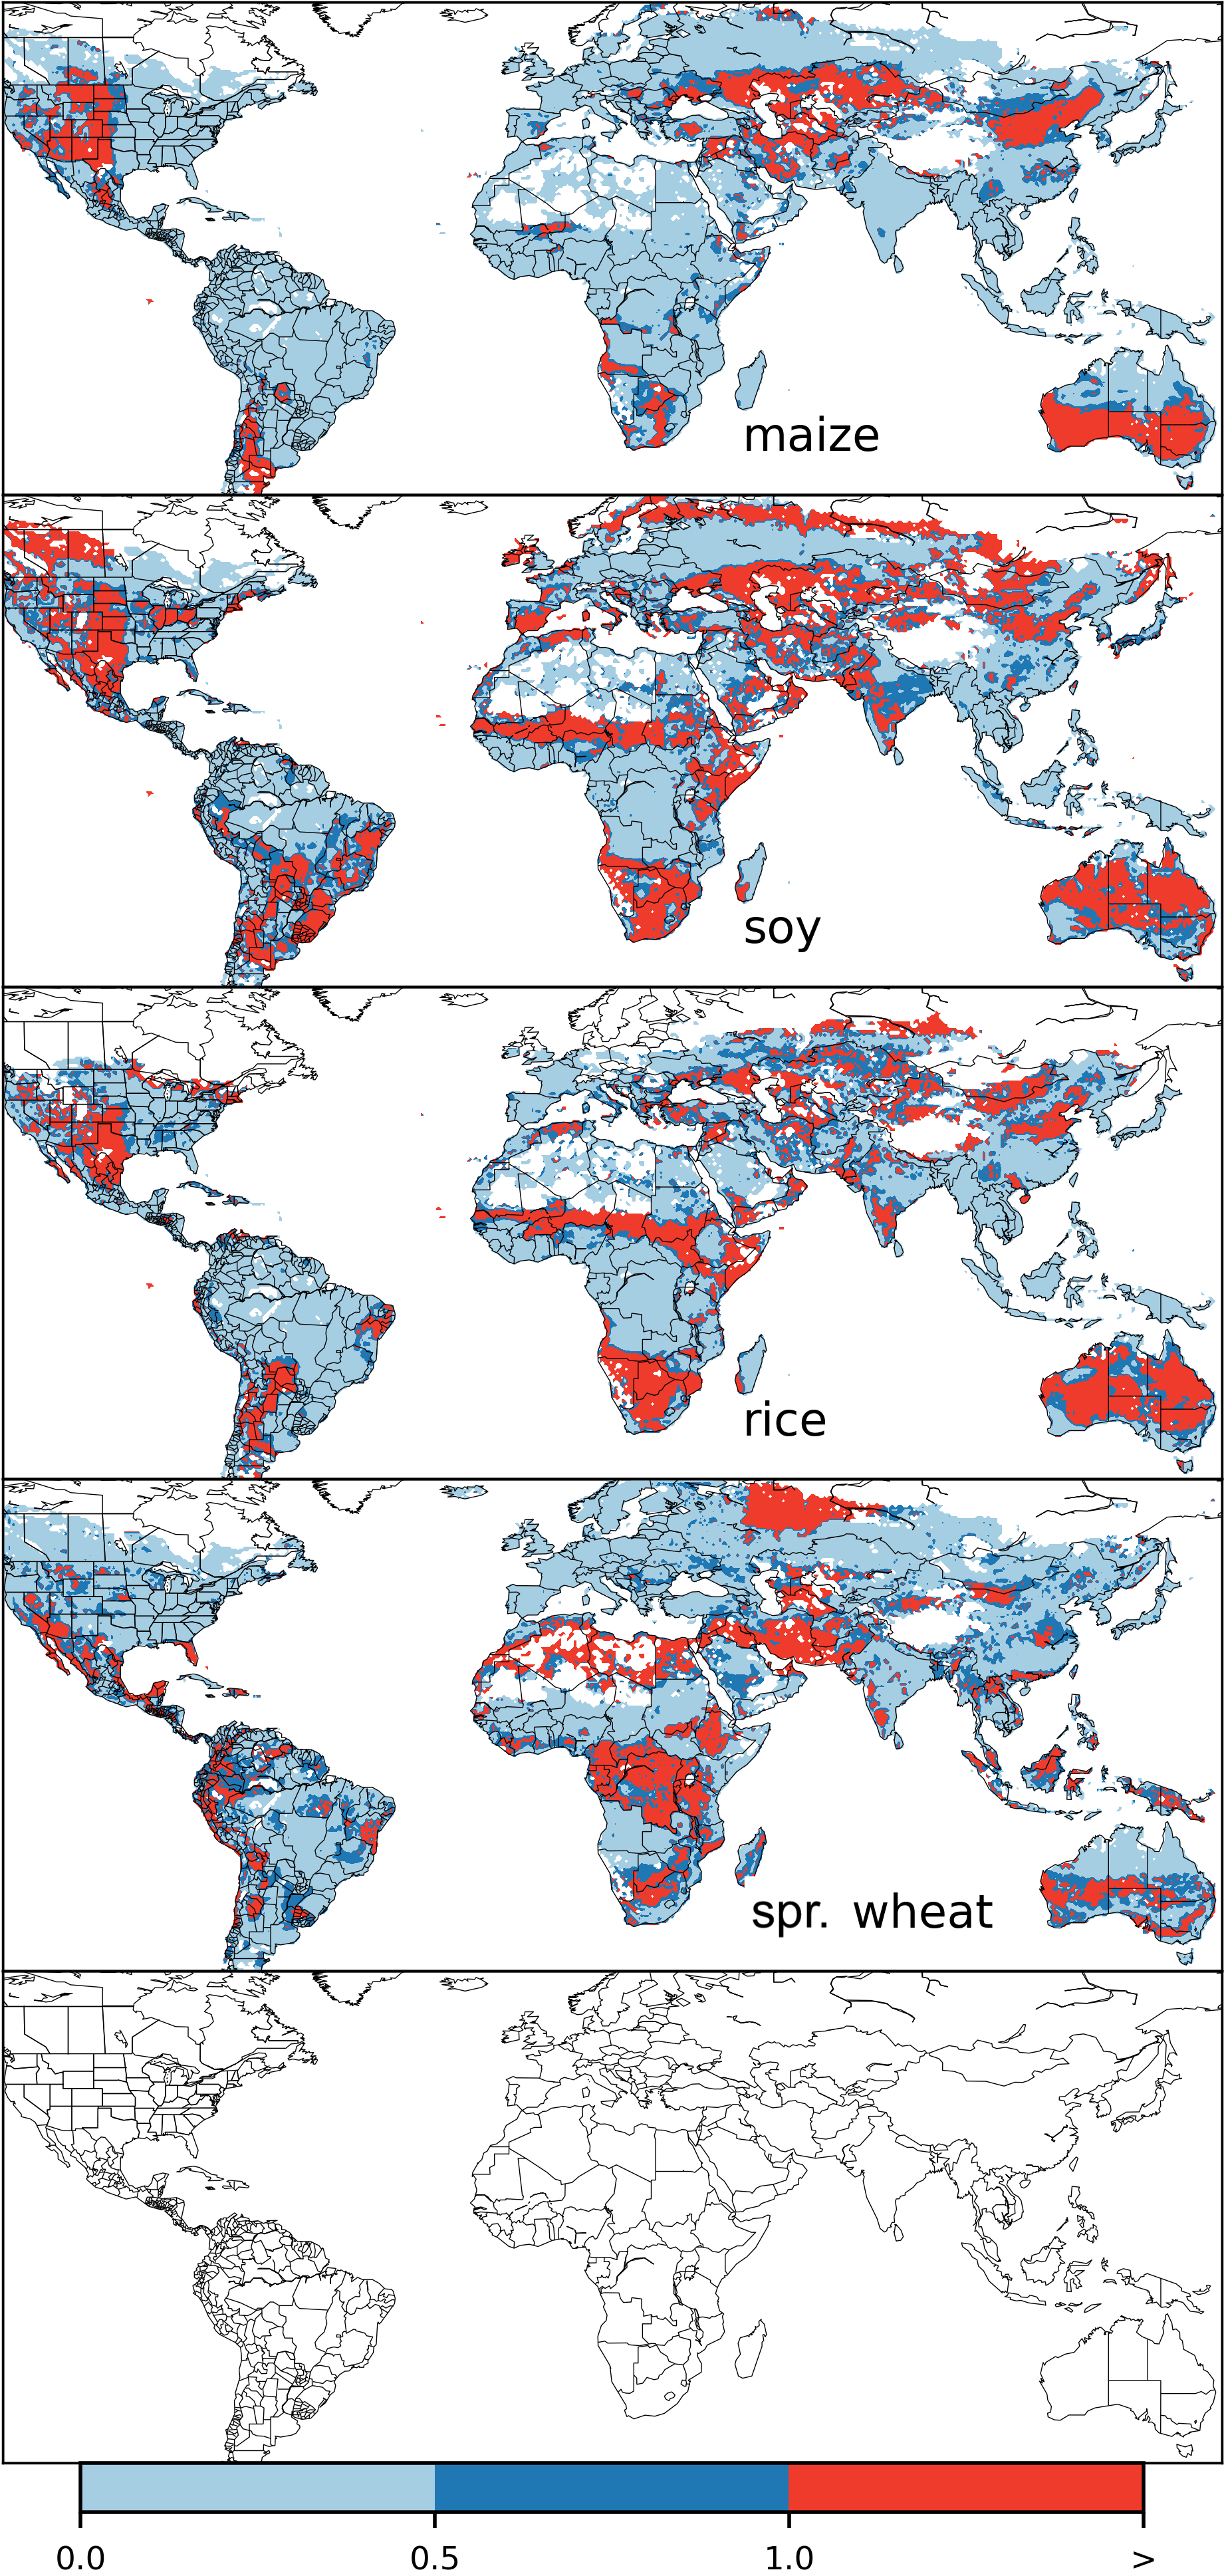
\includegraphics[width=\textwidth]{s_em_err_JULES.png}\\
    \caption{Illustration  of  our  test  of  emulator  performance,  applied  to  the JULES model for the T +4 scenario for rain-fed crops.  Contour colors indicate the normalized emulator error e, where e less than 1 means that emulator error exceeds the multi-model standard deviation. White areas are those where crops are not simulated by this model. Models differ in their areas omitted, meaning the number of samples used to calculate the multi-model standard deviation is not spatially consistent in all locations.}
    \label{fig:errorjules}
\end{minipage}
\hspace{.05\linewidth}
\begin{minipage}{.45\textwidth}
    \centering
    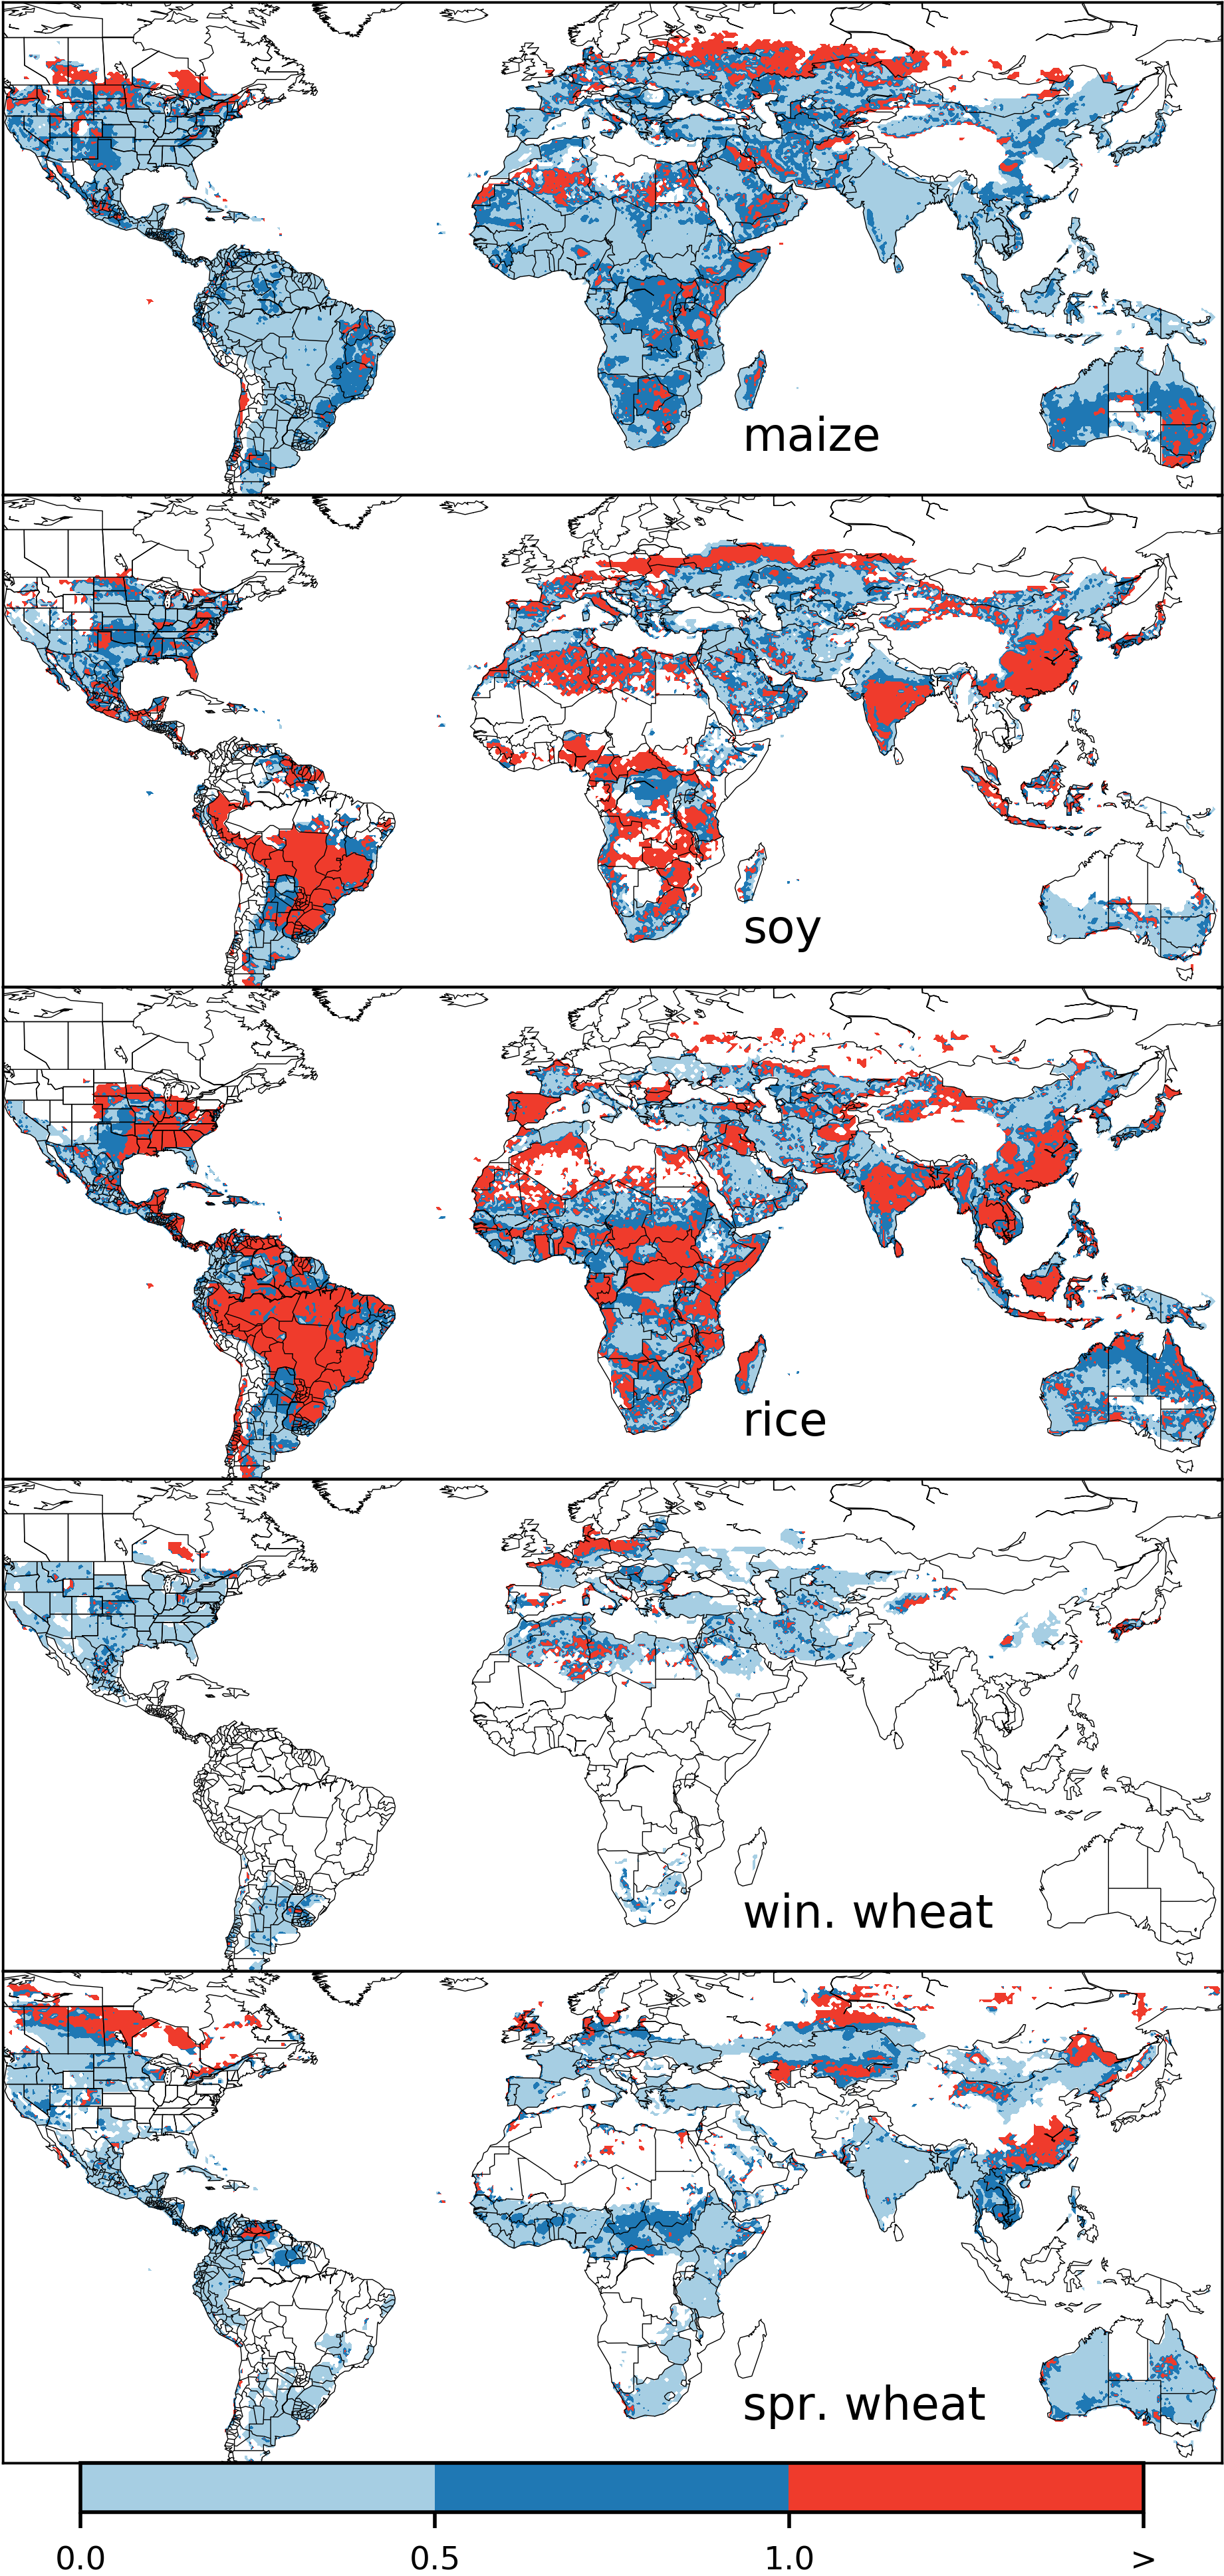
\includegraphics[width=\textwidth]{s_em_err_PROMET.png}
    \caption{Illustration of our test of emulator performance,  applied  to  the PROMET model for the T +4 scenario for rain-fed crops.  Contour colors indicate the normalized emulator error e, where e less than 1 means that emulator error exceeds the multi-model standard deviation. White areas are those where crops are not simulated by this model. Models differ in their areas omitted, meaning the number of samples used to calculate the multi-model standard deviation is not spatially consistent in all locations.}
    \label{fig:errorpromet}
\end{minipage}
\end{figure}

\clearpage
\section{Emulator results}
Example damage functions over the the four dimensions included in the study. All crops shown and split by KG climate regions. 

\begin{figure}[h!]
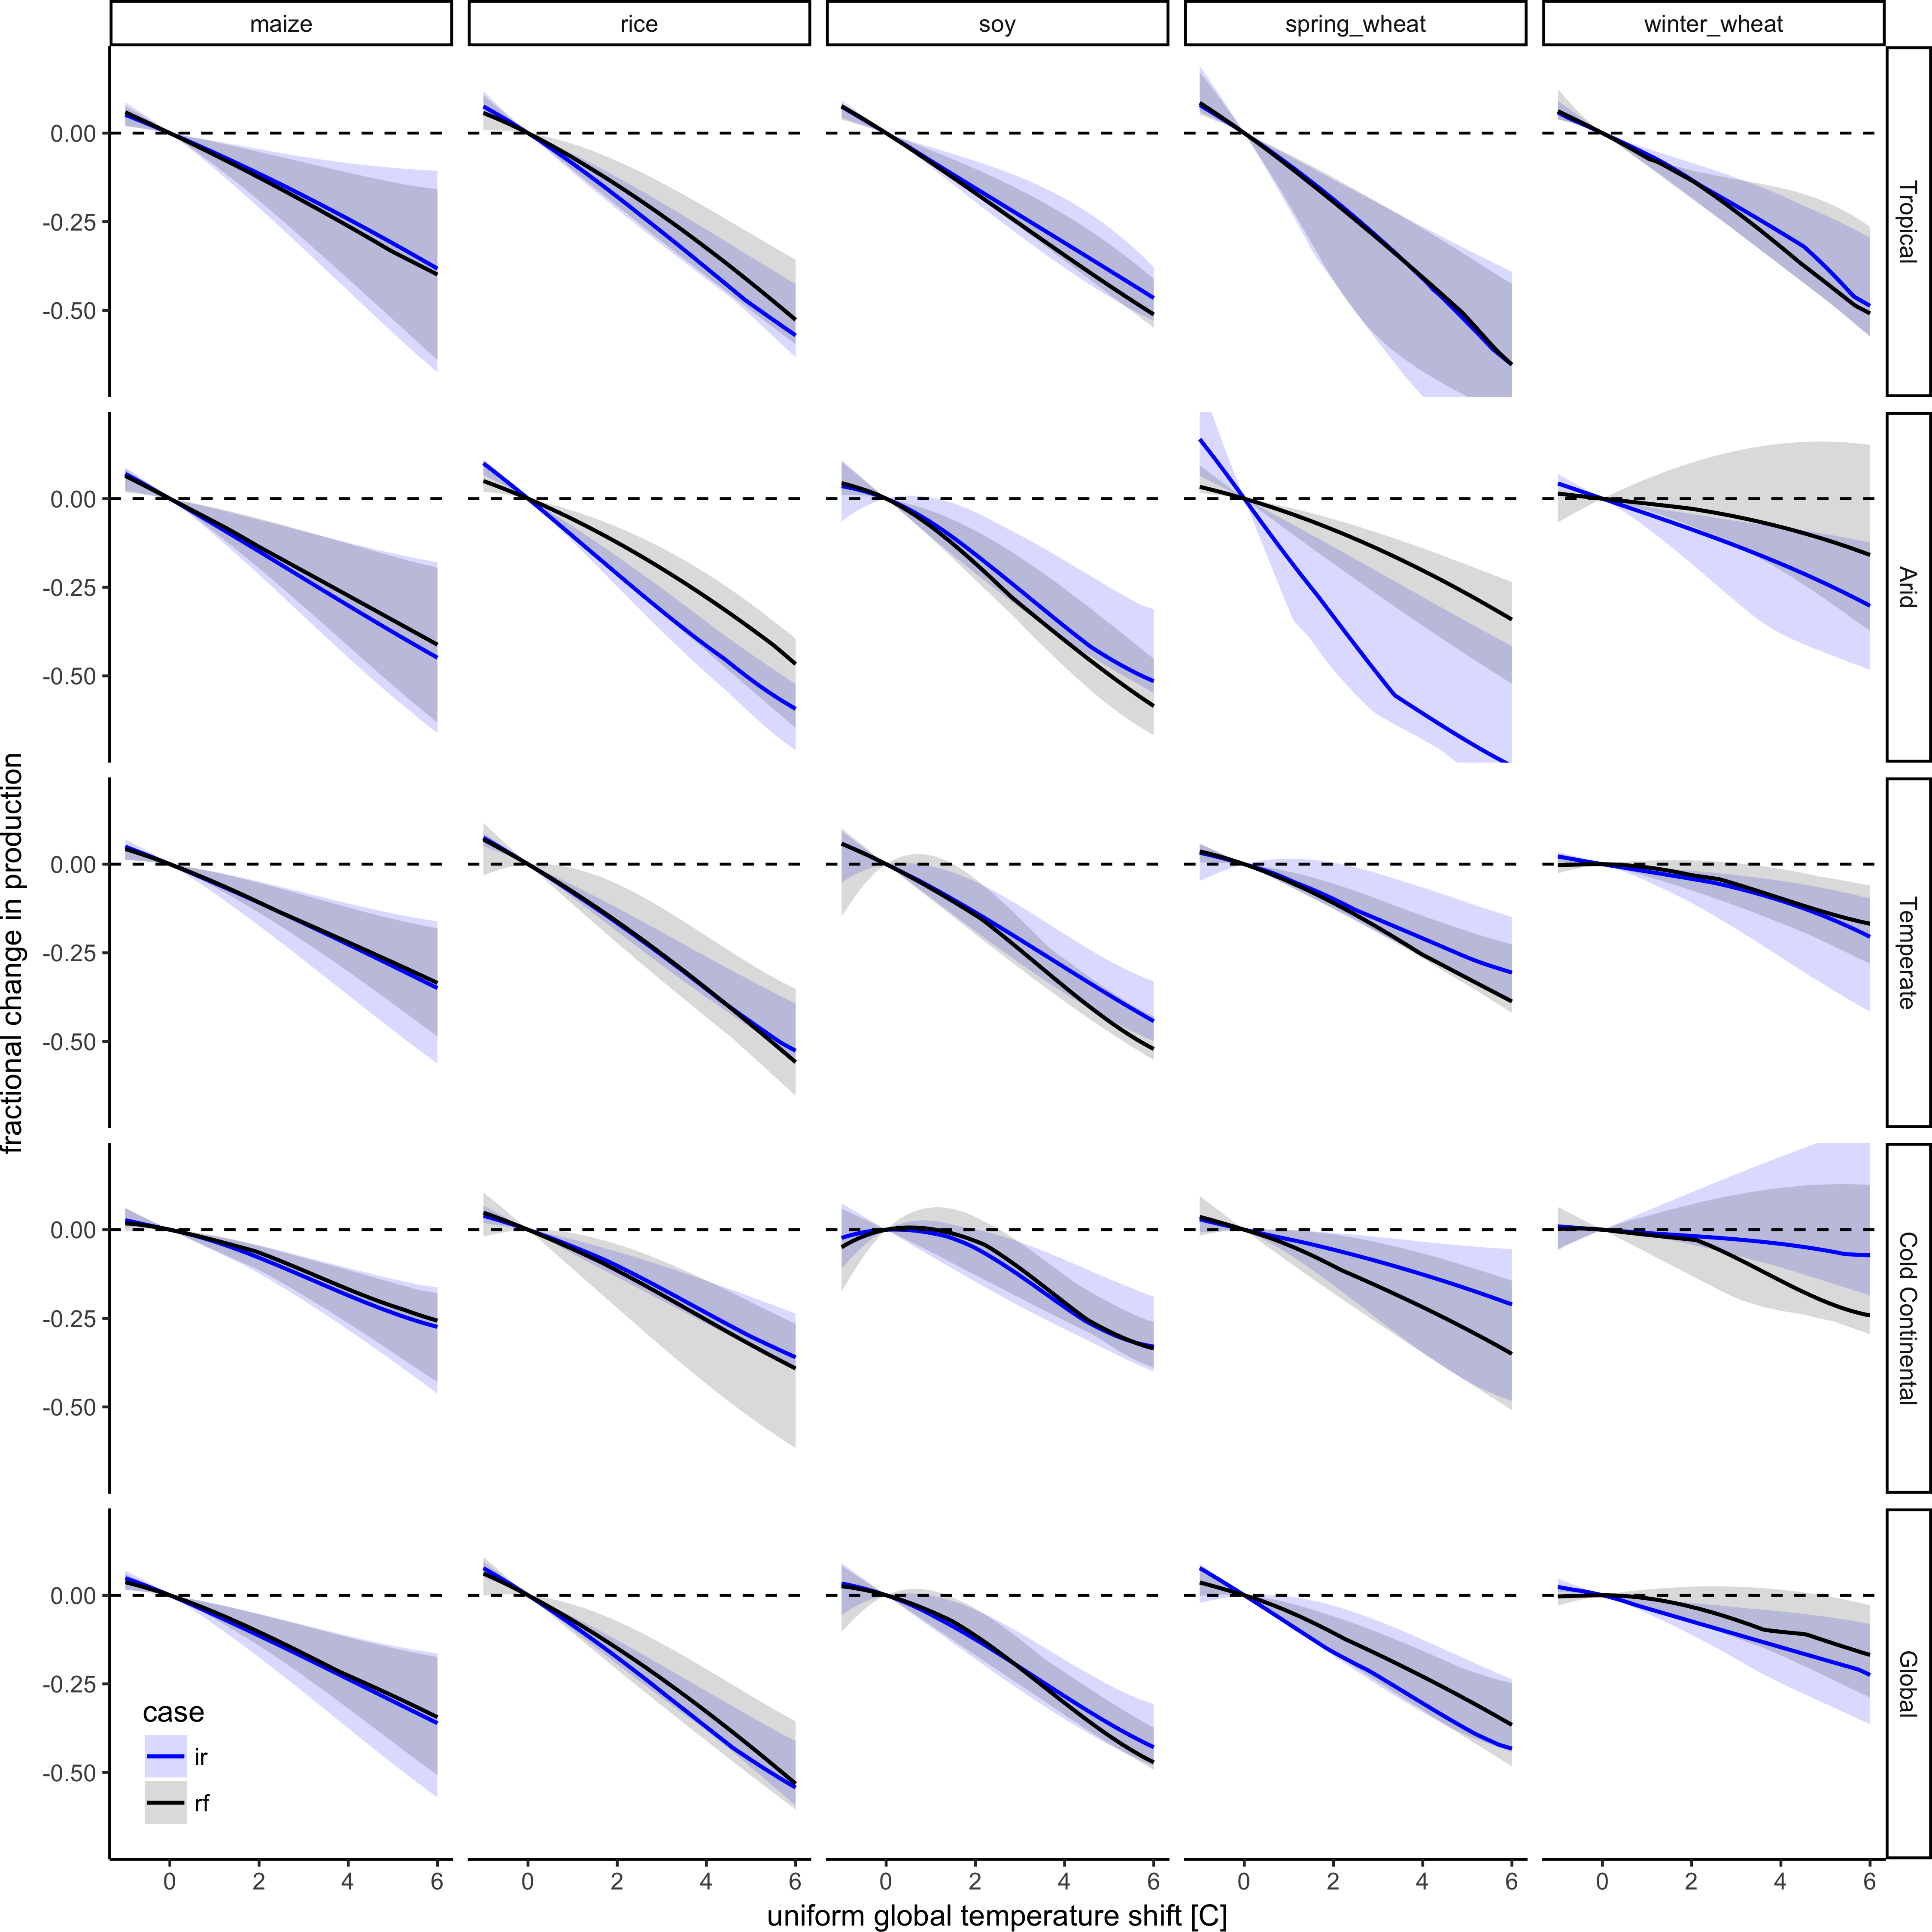
\includegraphics[width=\textwidth]{s_temp.png}\\
\caption{Multi-model ensemble spread in sensitivity to changes in the temperature dimension. 5\% median and 95\% percentile emulated damage function for currently cultivated areas. Irrigated and rain-fed crops shown. PROMET and JULES removed from ensemble. All other covariates held constant. Uniform temperature shift should not be interpreted as a realistic climate change.}
\label{fig:temperature}
\end{figure}

\begin{figure}[h!]
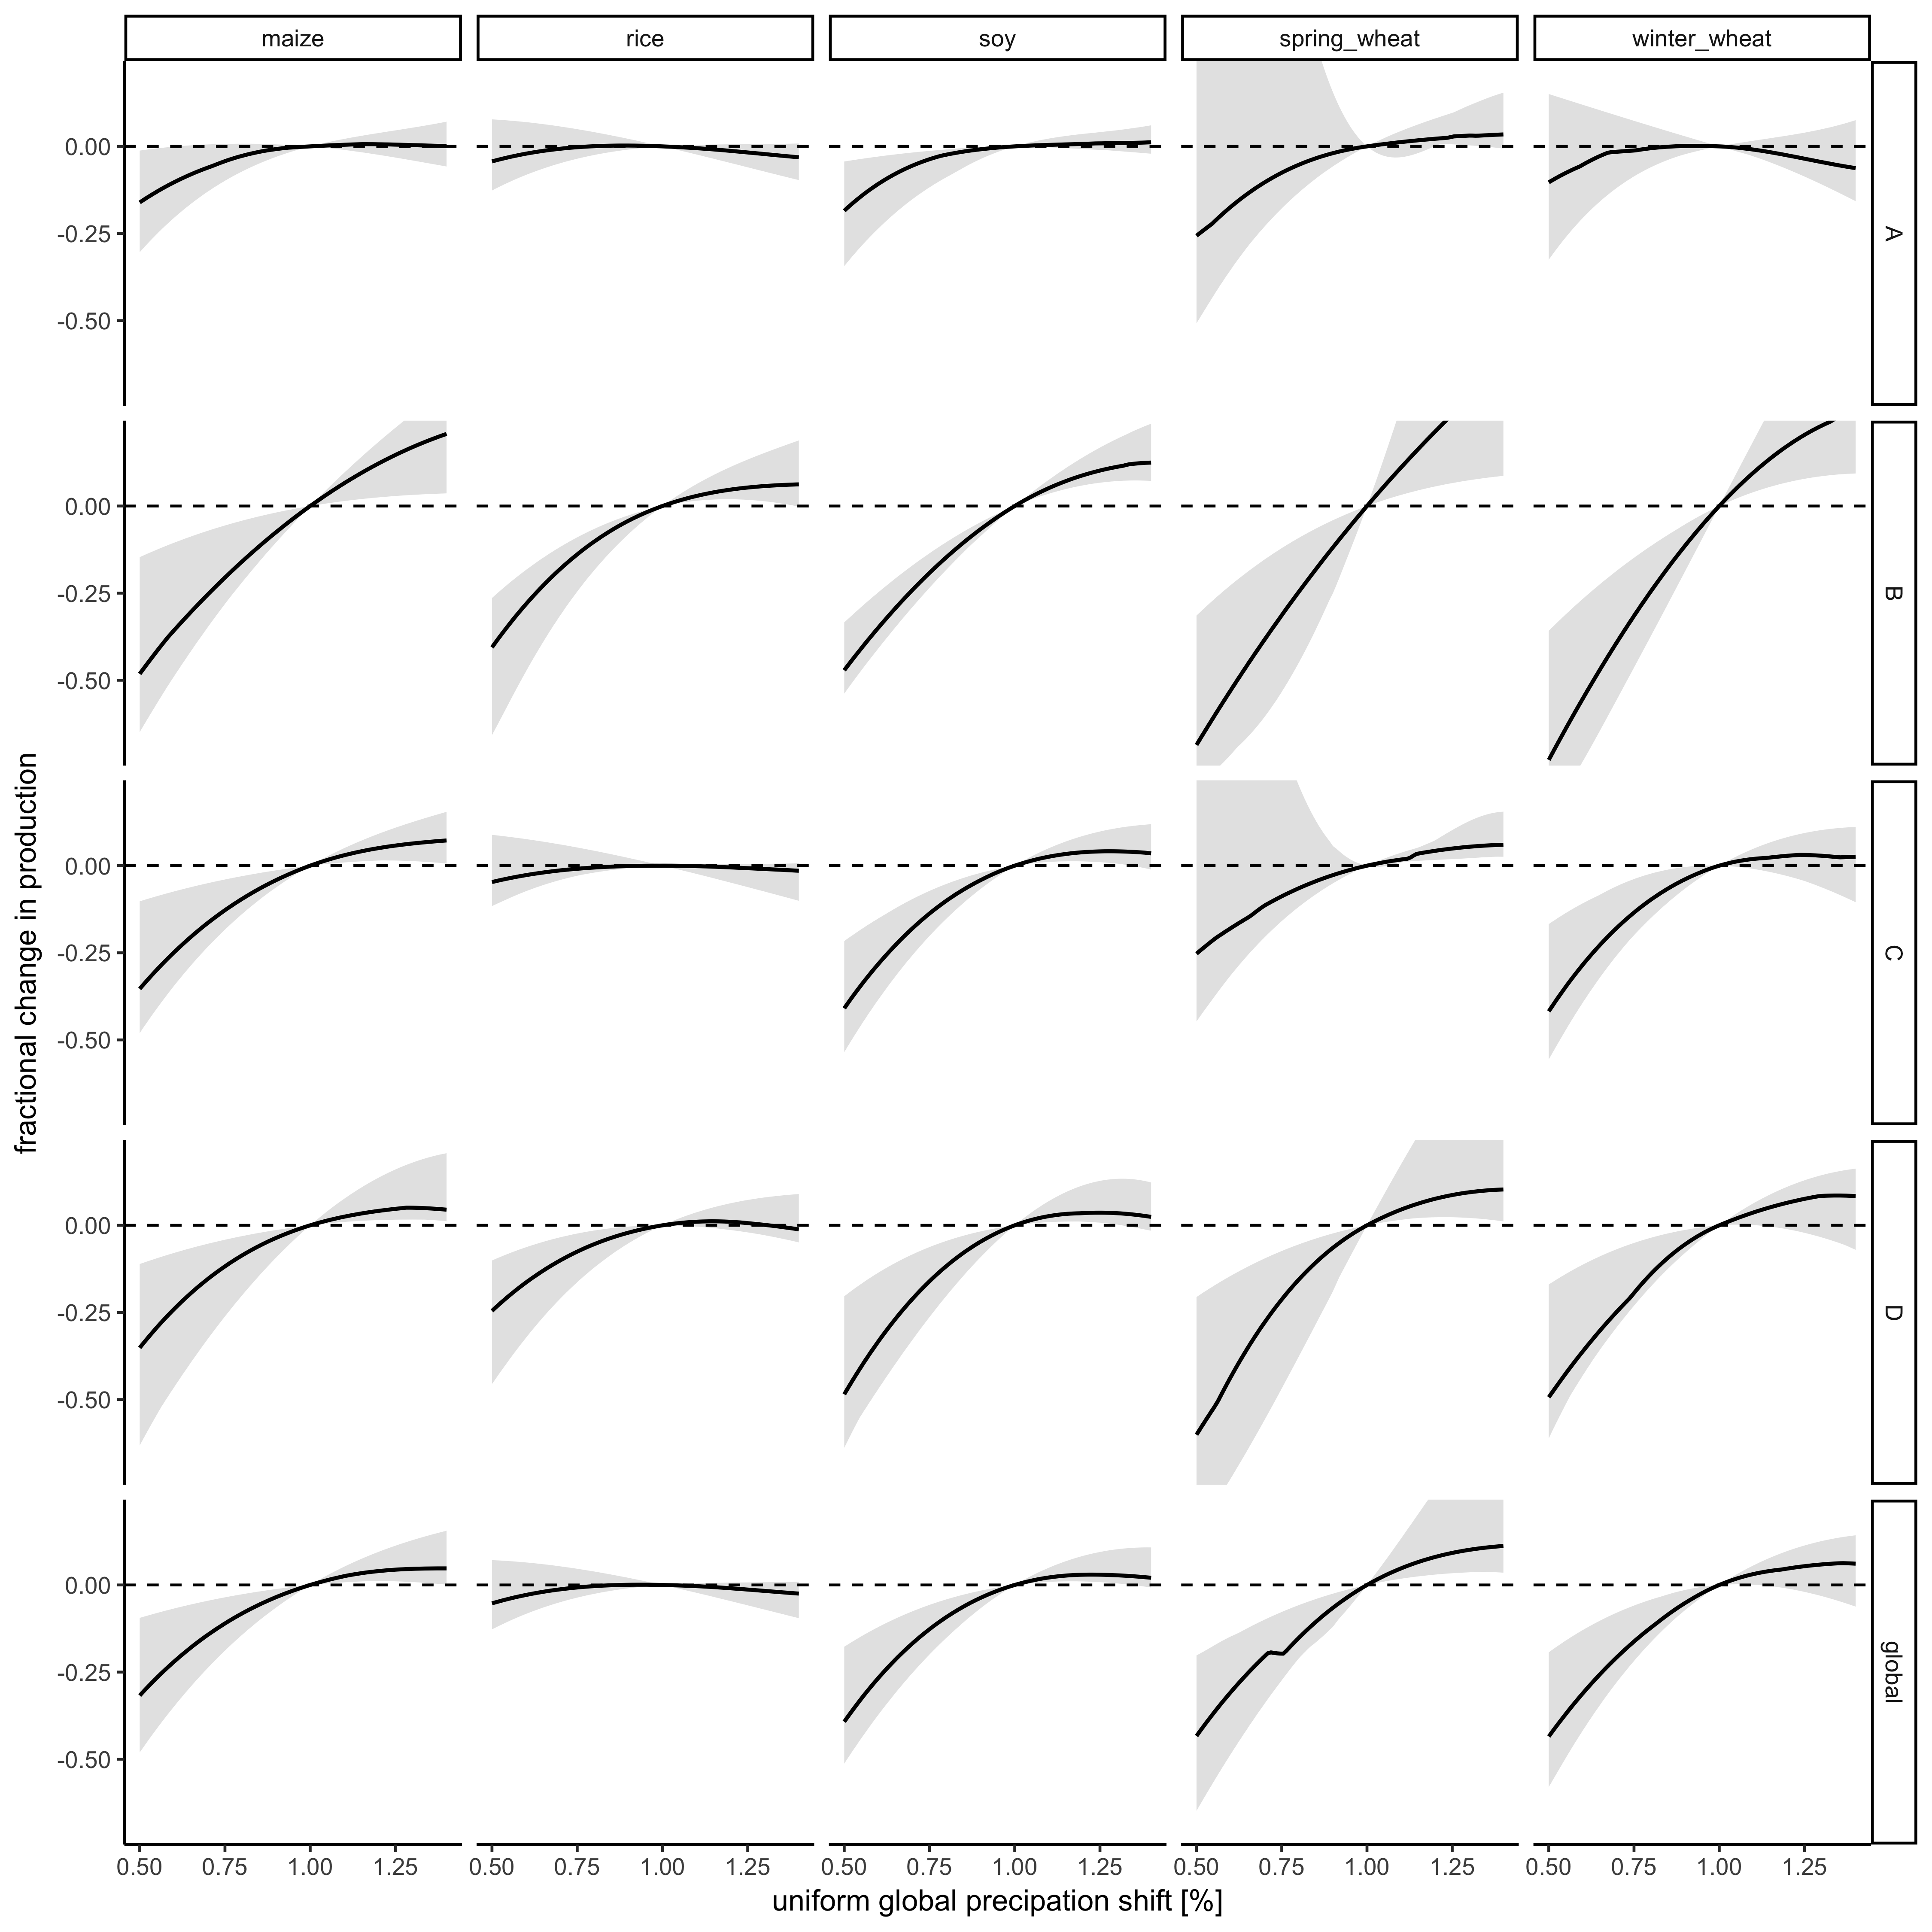
\includegraphics[width=\textwidth]{s_water.png}\\
\caption{Multi-model ensemble spread in sensitivity to changes in the water dimension. 5\% median and 95\% percentile emulated damage function for currently cultivated areas. PROMET and JULES removed from ensemble. All other covariates held constant. Uniform precipitation shift should not be interpreted as a realistic climate change.}
\label{fig:water}
\end{figure}

\begin{figure}[h!]
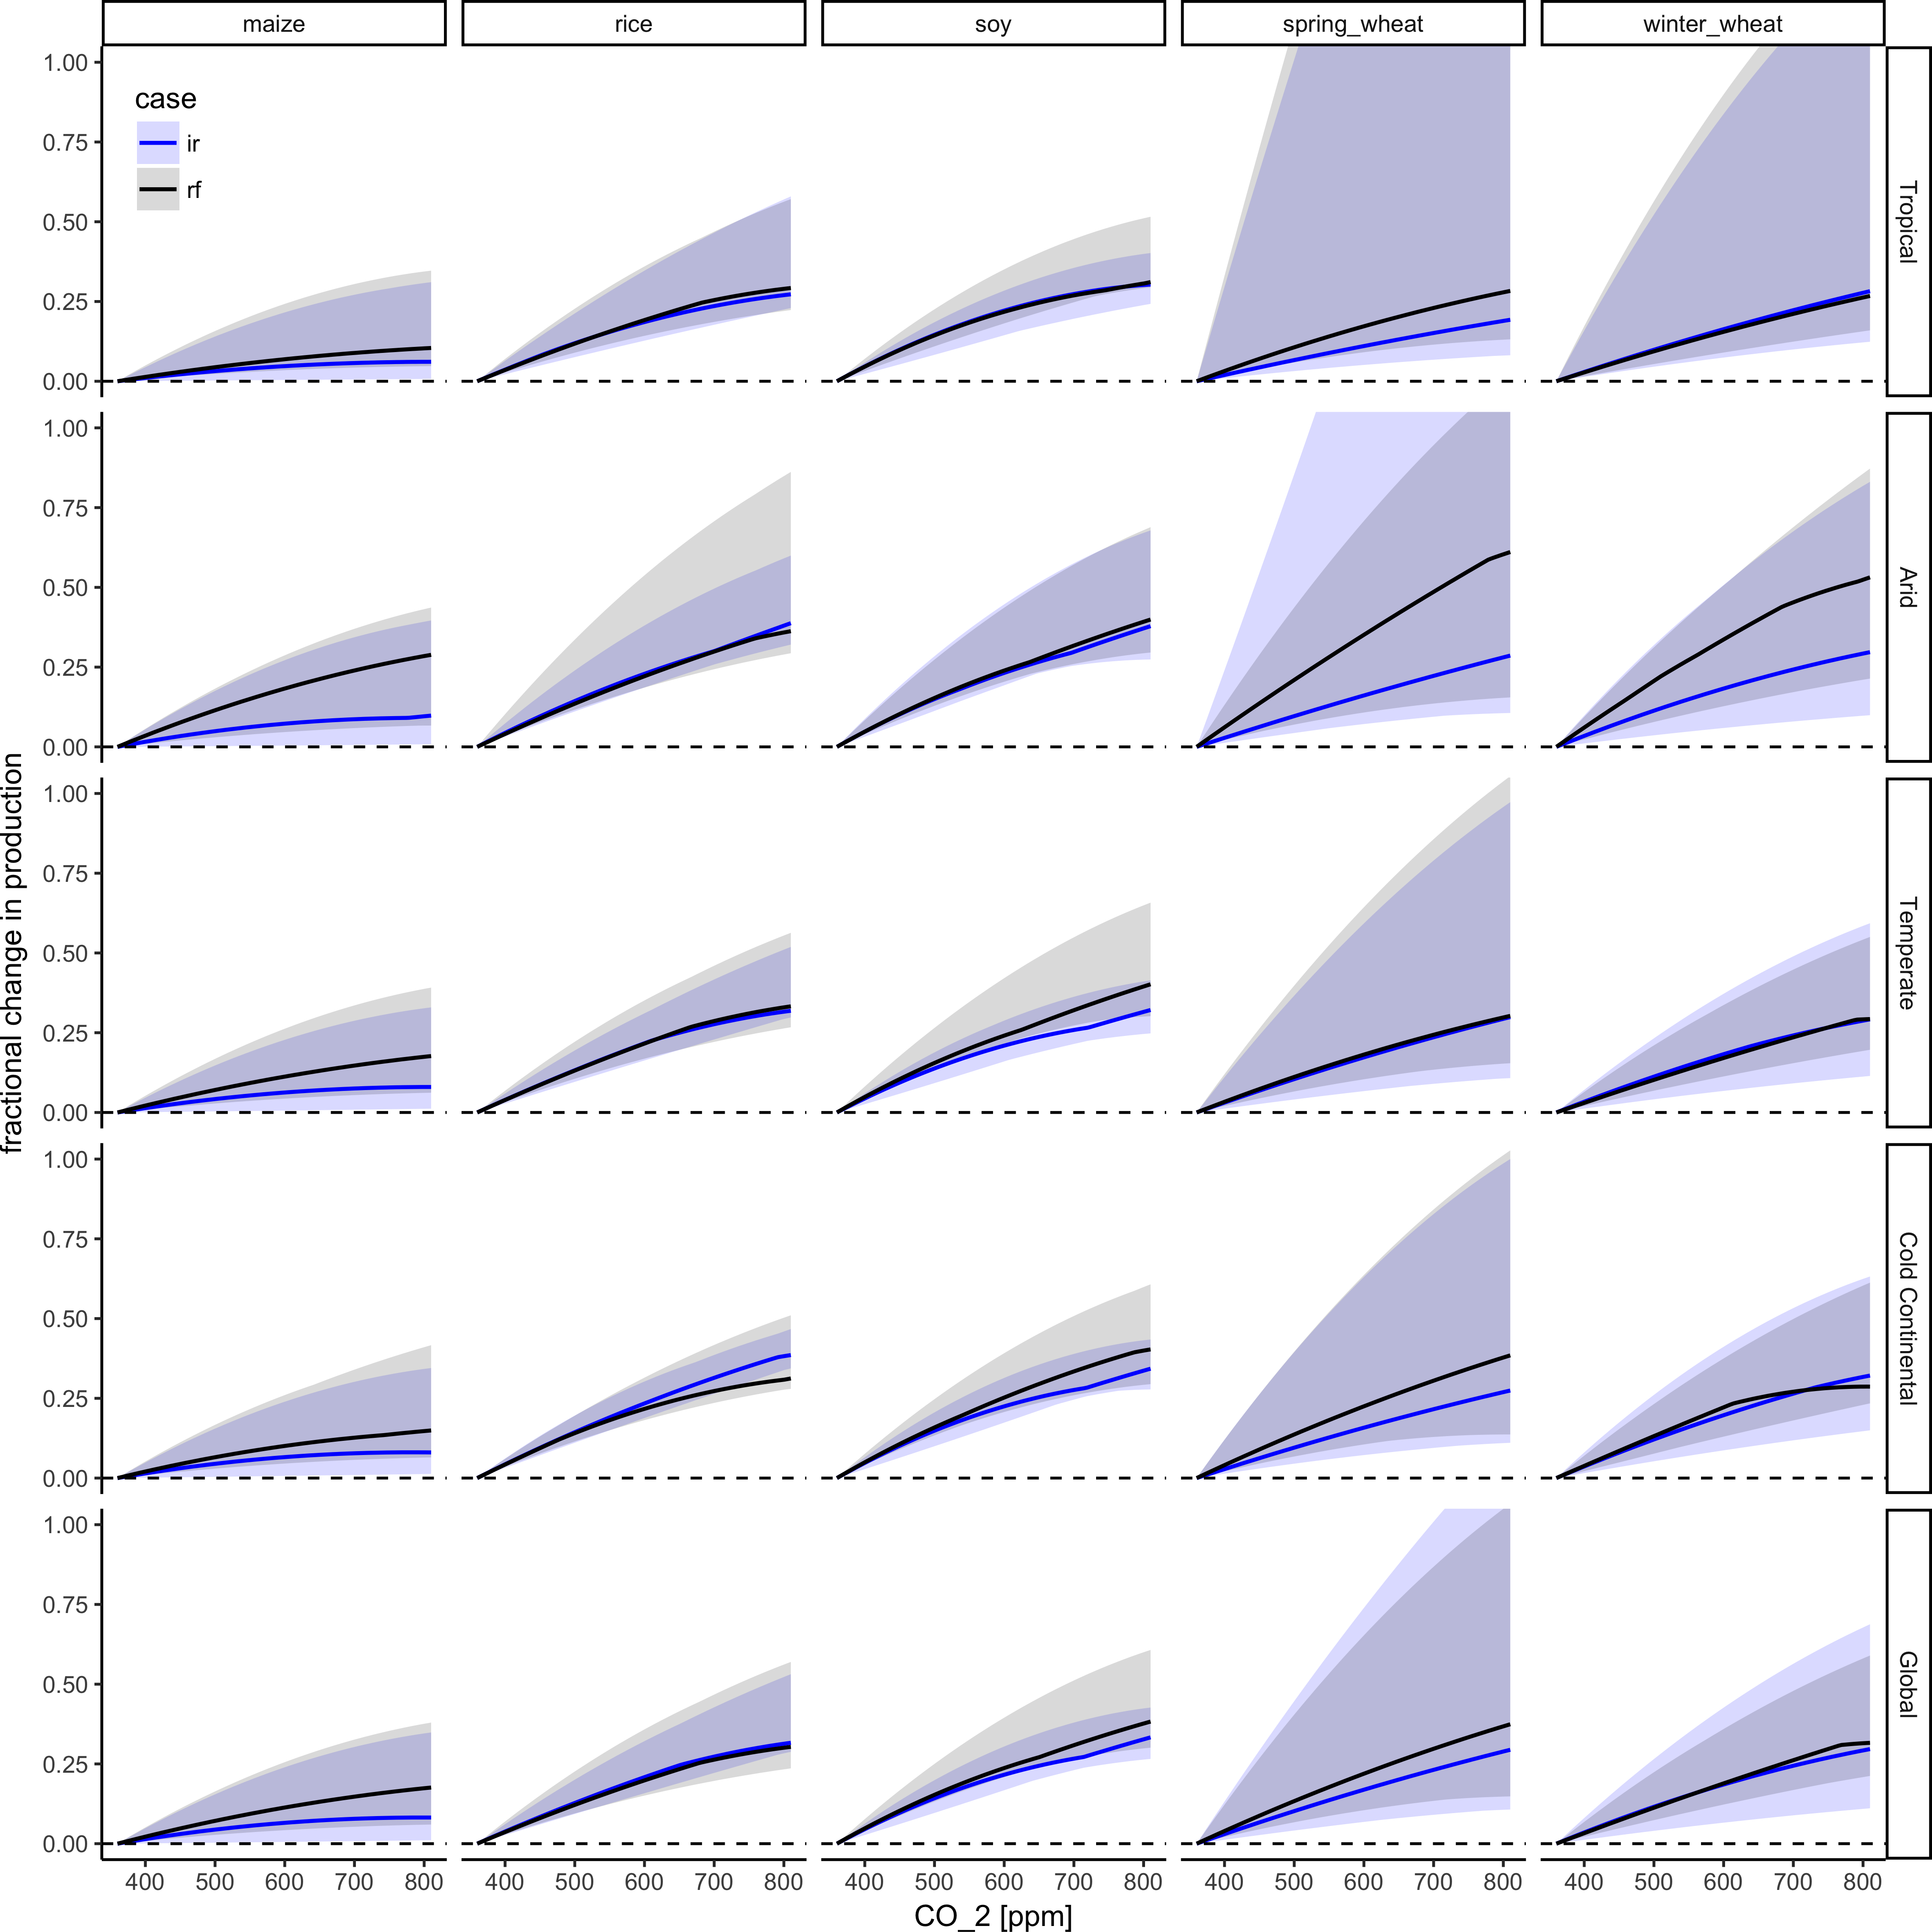
\includegraphics[width=\textwidth]{s_carbon.png}\\
\caption{Multi-model ensemble spread in sensitivity to changes in the carbon dimension. 5\% median and 95\% percentile emulated damage function for currently cultivated areas. Irrigated and rain-fed crops shown. PROMET and JULES removed from ensemble. All other covariates held constant.}
\label{fig:carbon}
\end{figure}

\begin{figure}[h!]
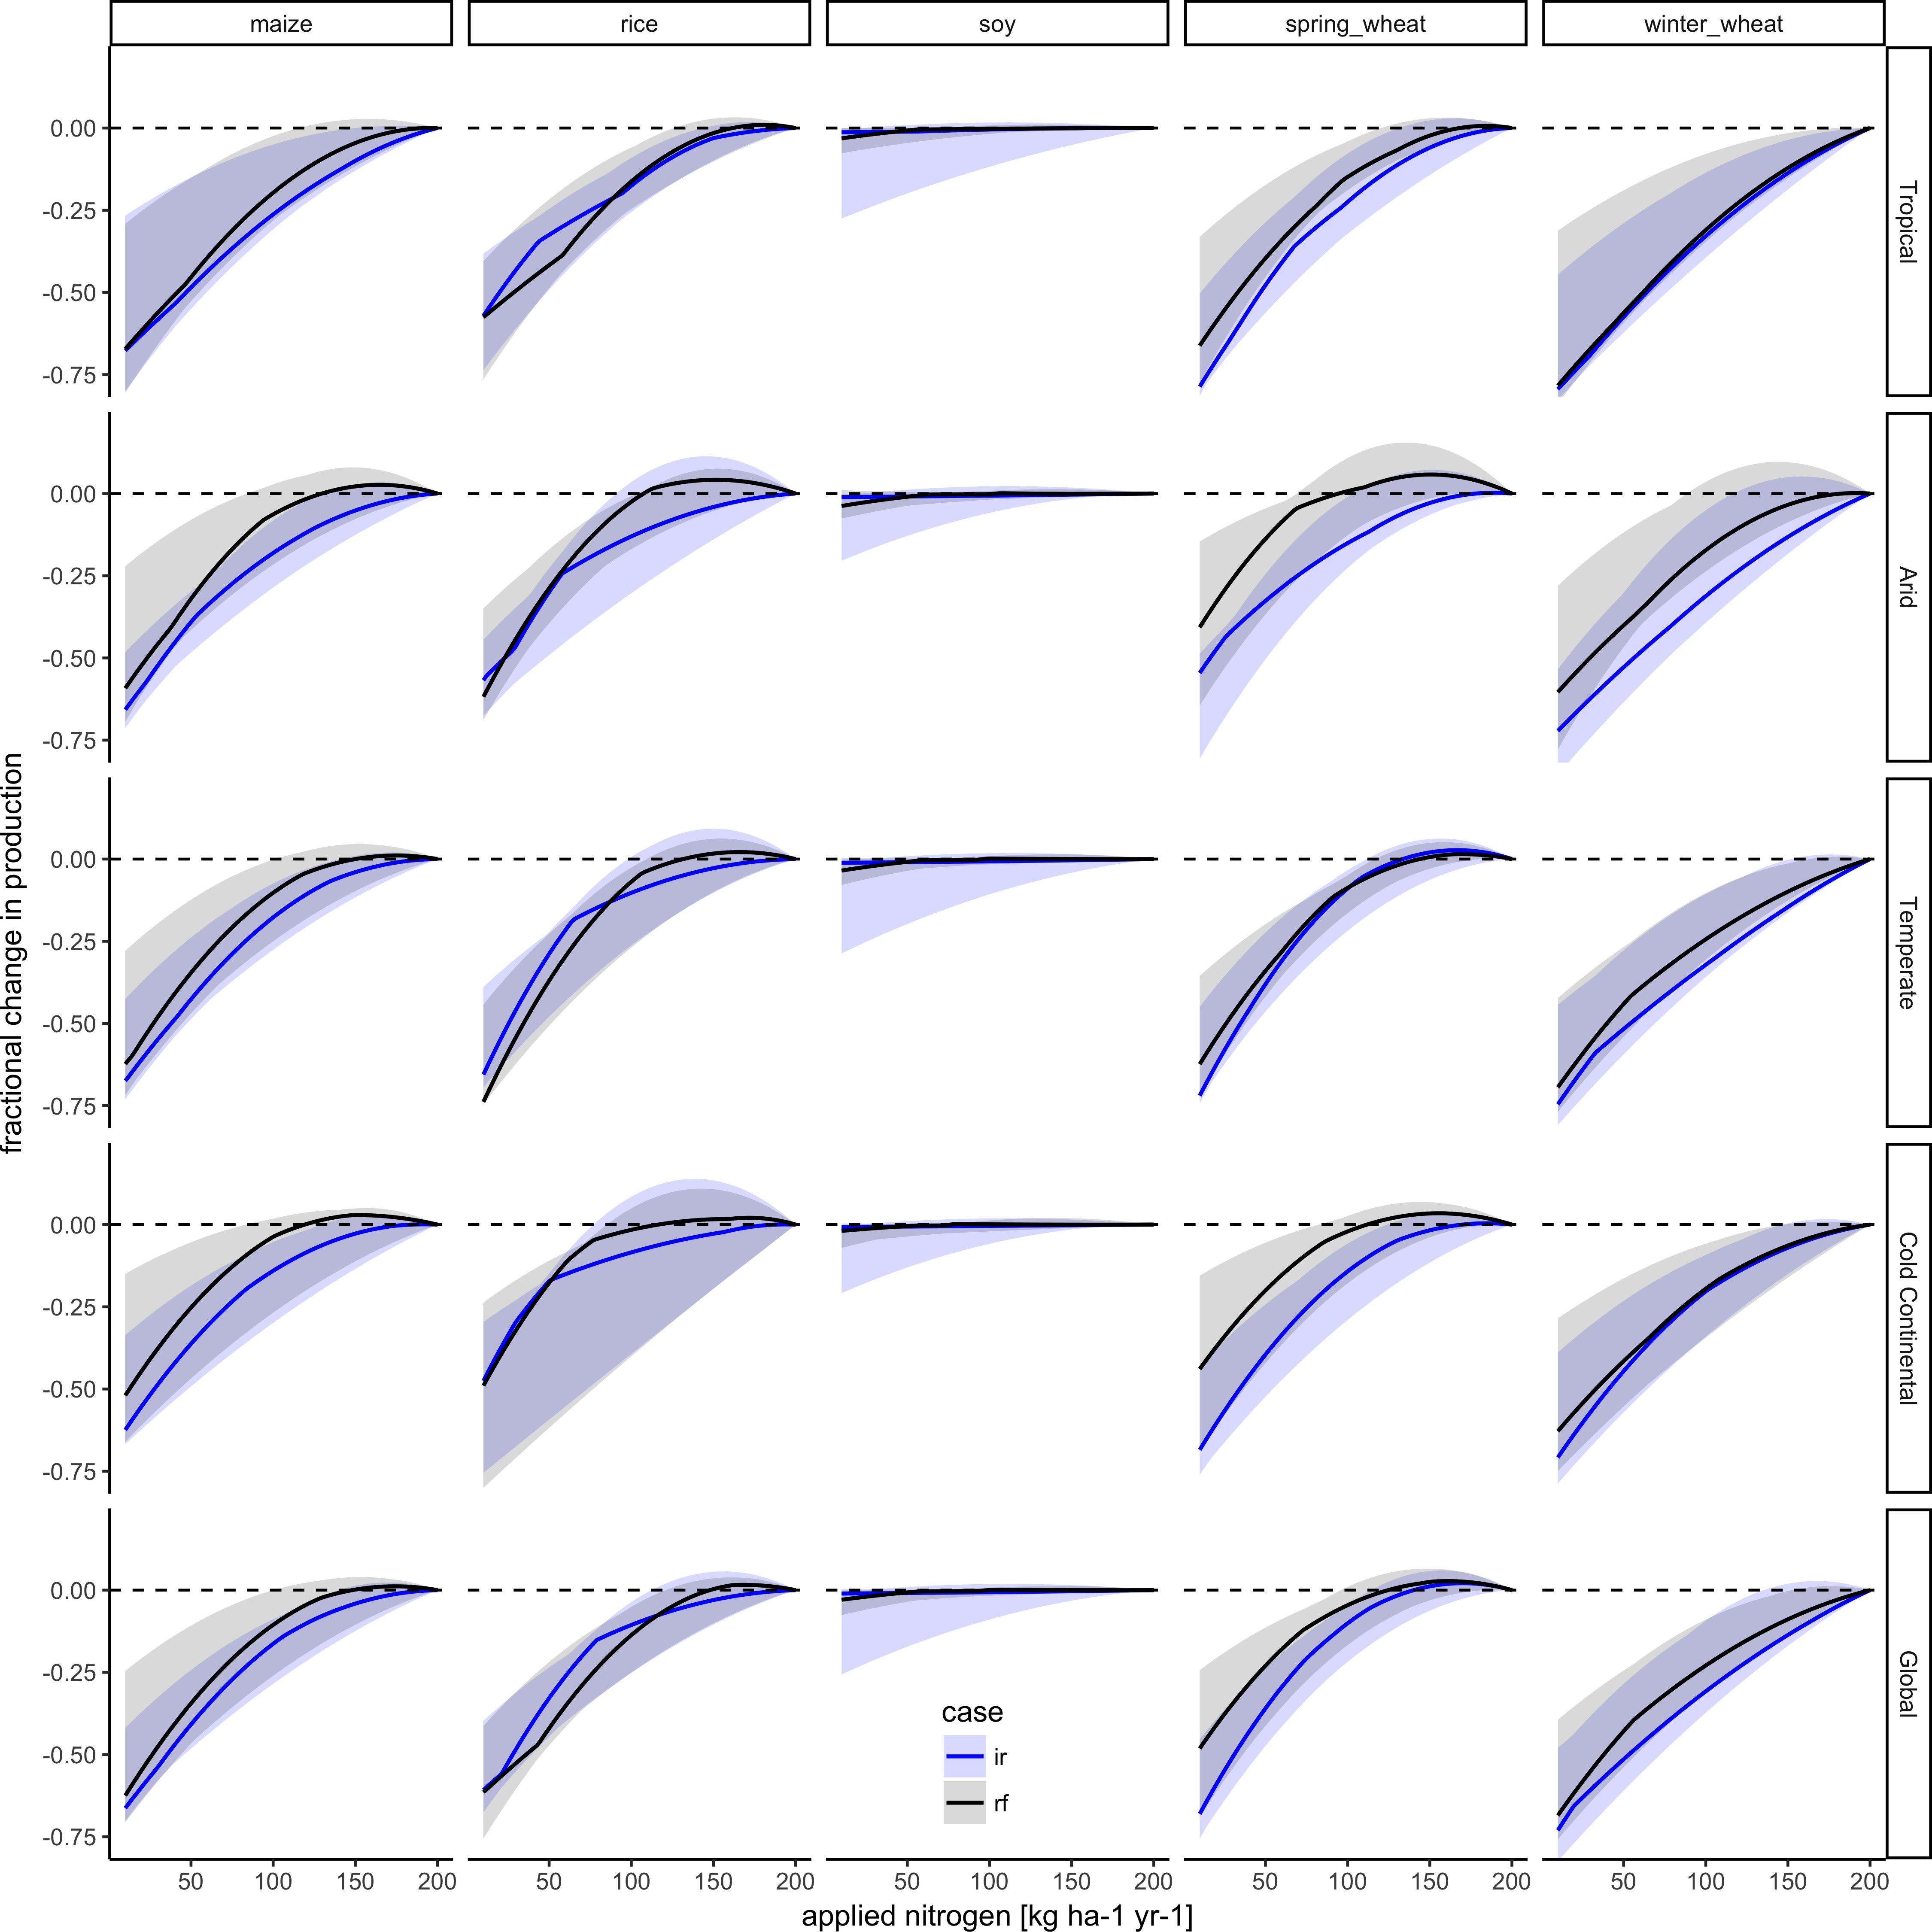
\includegraphics[width=\textwidth]{s_nitrogen.png}\\
\caption{Multi-model ensemble spread in sensitivity to changes in the nitrogen dimension. 5\% median and 95\% emulated damage function for currently cultivated areas. Irrigated and rain-fed crops shown. PROMET and JULES removed from ensemble. All other covariates held constant. Soy shows the lowest sensitivity to Nitrogen as expected. Irrigated crops are more sensitive to low Nitrogen}
\label{fig:nitrogen}
\end{figure}

\begin{figure}[h!]
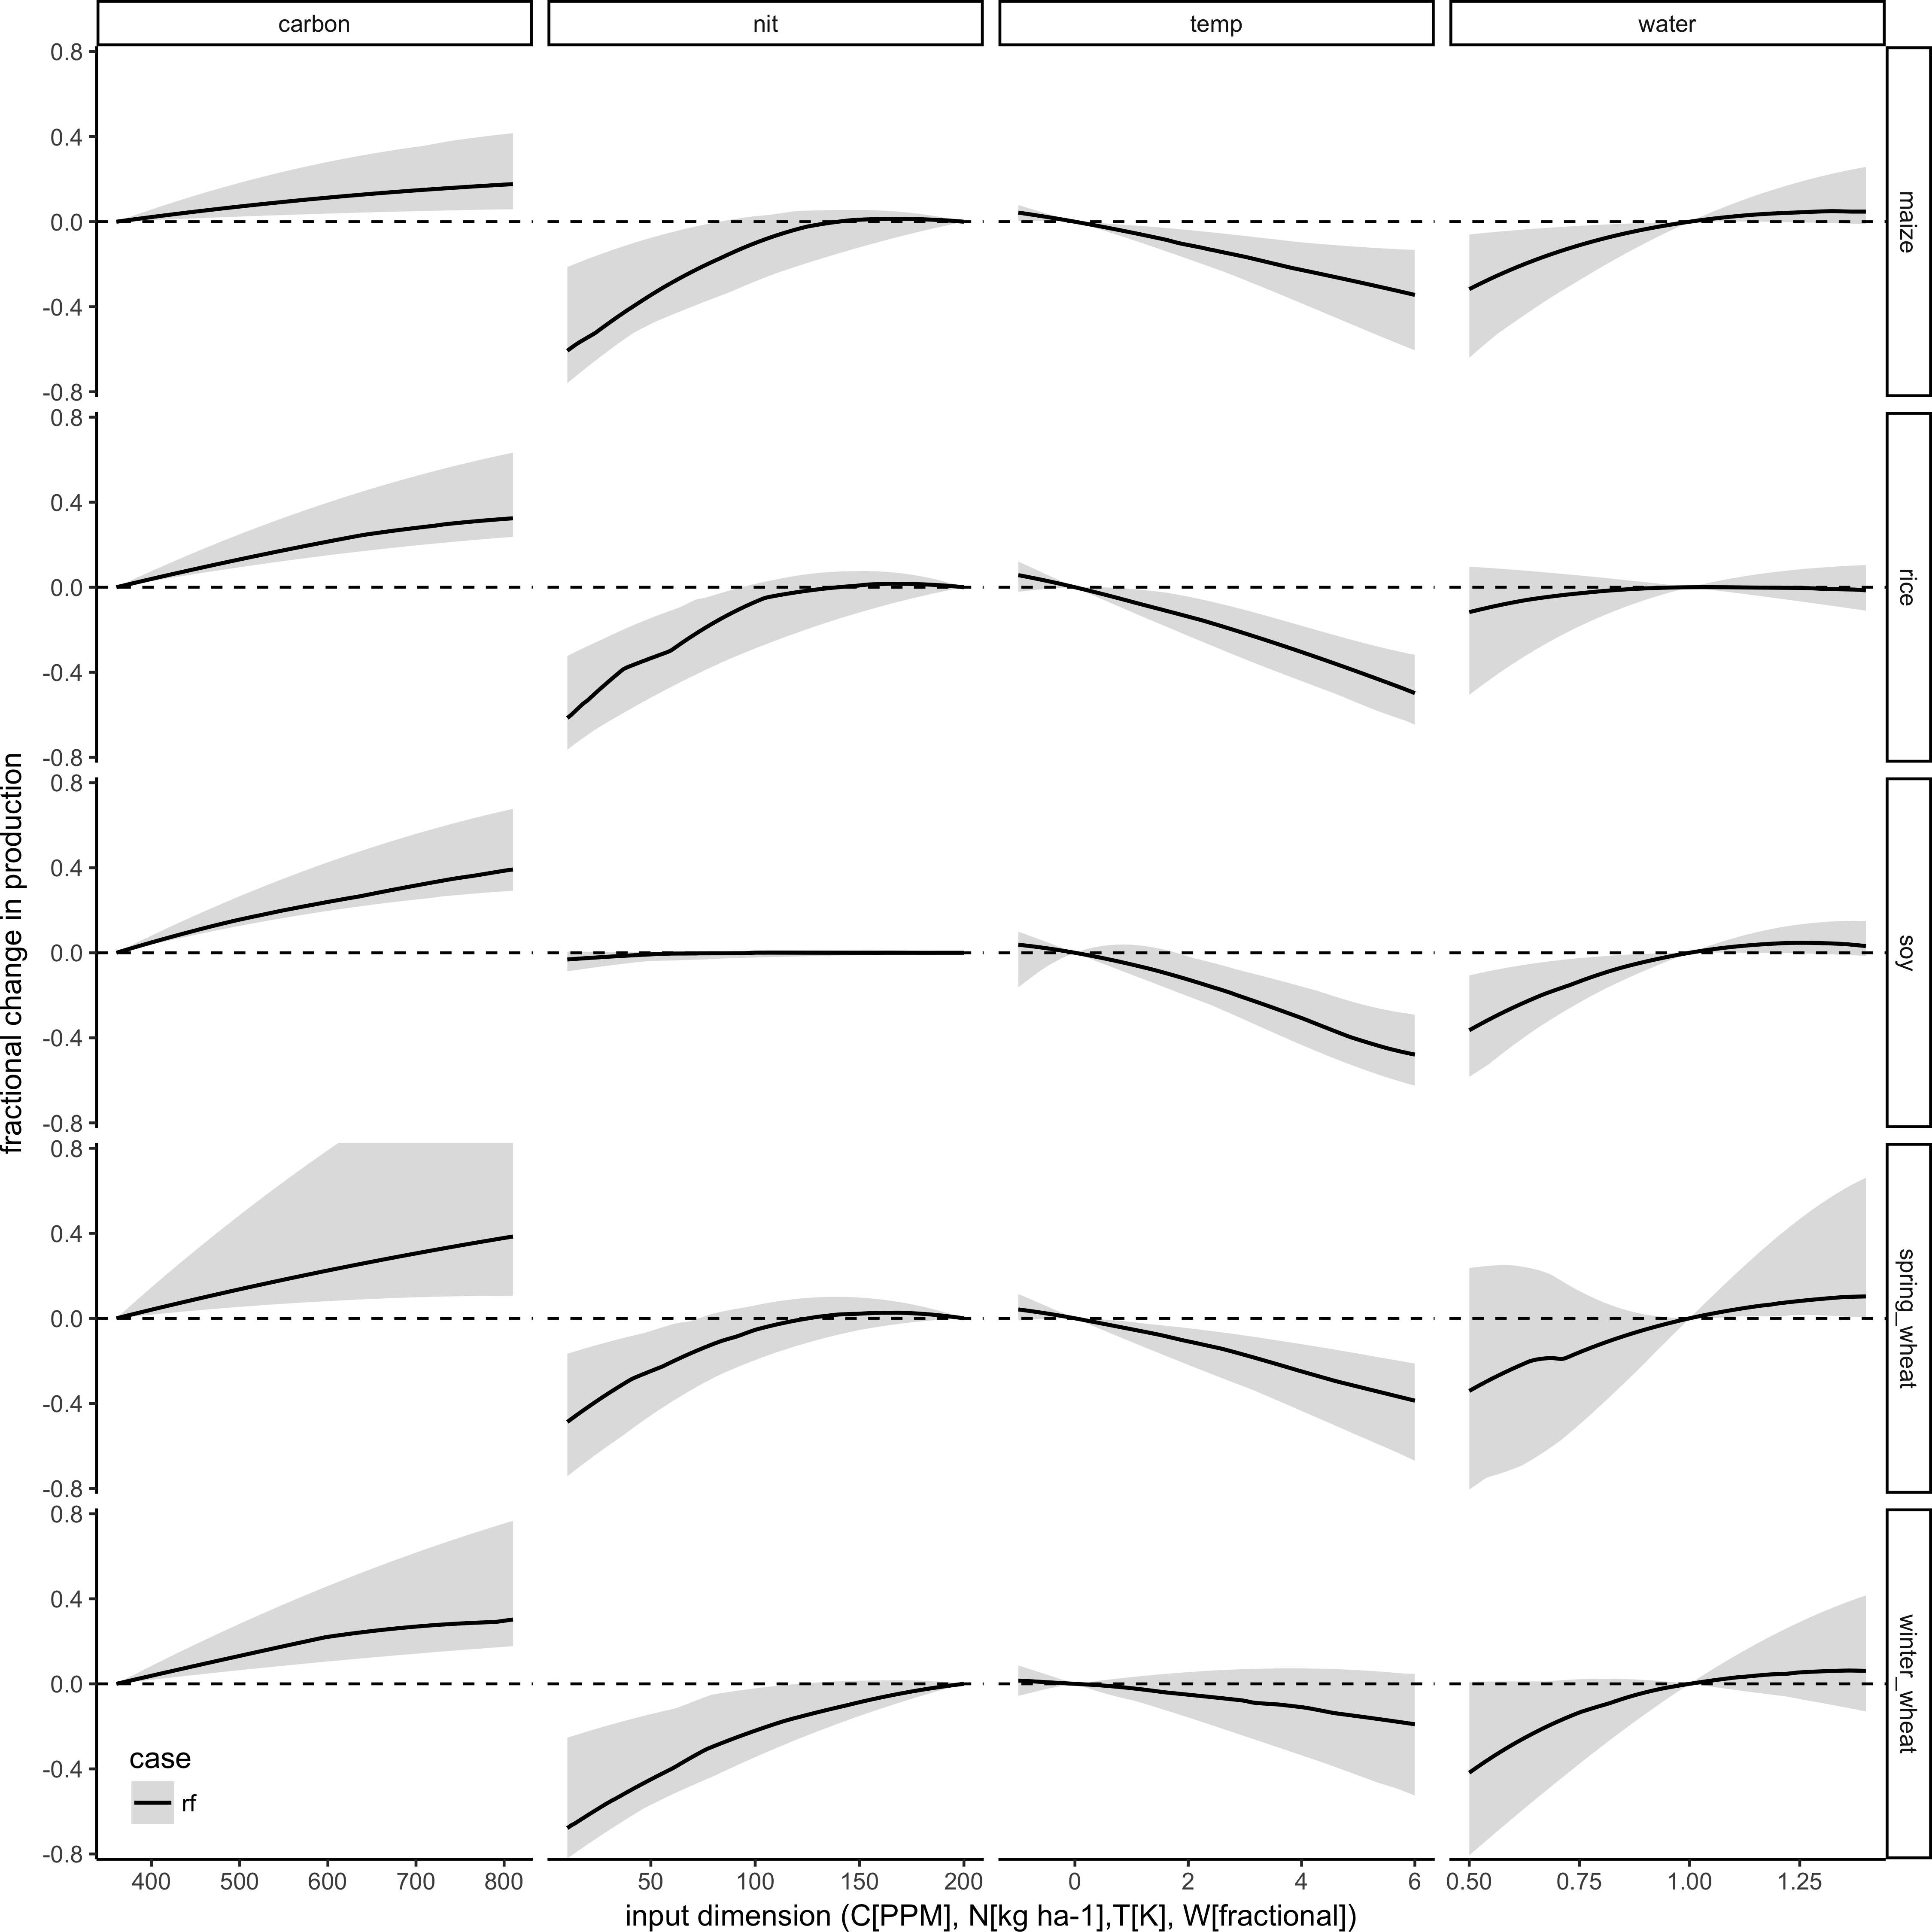
\includegraphics[width=\textwidth]{em_CTWN_all_crops.png}\\
\caption{Multi-model ensemble spread in sensitivity to changes in all four dimensions for rain-fed crops at the global level. 5\% median and 95\% percentile emulated damage function for currently cultivated areas. PROMET and JULES removed from ensemble. All other covariates held constant in each case.}
\label{fig:all_dims}
\end{figure}

\clearpage
\bibliography{bib.bib}

\end{document}
